% Chapter 6

\chapter{ Examples }
\label{Chapter6}
\lhead{Chapter 6. \emph{ Examples }}

\section{Forward rendering}
\label{sec:ForwardRenderingExample}

Forward rendering is the classical algorithm utilized since the very beginning of rasterization and definitely the most commonly used one thus far. Since the introduction of GeForce 256 in late 1999, it has had special hardware and API support in consumer graphics devices. The special support is only being phased out recently due to programmable shading's ability of supporting the whole forward rendering algorithm efficiently. While modern rendering APIs such as \emph{Direct3D 10} and \emph{OpenGL 3.1's Core profile} no longer have dedicated support for transformation and lighting, the algorithm is still widely used and implemented via shaders. Despite other rendering algorithms being available, the performance characteristics of the forward approach make it favorable in many circumstances, hence it's imperative that Nucleus provides out of the box support for it.

The basic outline of the forward rendering algorithm is as follows:
	
\begin{algorithmic}
\FOR{each $object$ \textbf{in} $scene$}
	\STATE $lights$ $\Leftarrow$ determine-lights-influencing($object$)
	\STATE $radiance \Leftarrow 0$
	\FOR{each $light$ \textbf{in} $lights$}
		\STATE $radiance \Leftarrow radiance$ + \textbf{illuminate}($object$, $light$)
	\ENDFOR
	\STATE $output(radiance)$
\ENDFOR
\end{algorithmic}

The inner loop iterating all lights influencing an object can either can be approached in severals ways, for instance via multi-pass rendering, accumulating light influences into a \emph{Spherical Harmonics}-based approximation, approximating multiple lights into a single ``best-fit'' source, etc. The implementation in Nucleus uses a relatively simple approach of summing the contributions per-pixel on the GPU.

Iteration over a dynamically-sized array of lights in the fragment shader is an option, however it may be observed that for each light set influencing an object, all pixels will take the same branches. Hence it's desirable to unroll the loops and conditionals. This is done by generating a specialized shader for each set of influencing lights and statically evaluating all contributions.

\subsection{Kernel graph generation}

Each object has a \emph{Structure}, a \emph{Material} and a \emph{Reflectance} kernel associated with it. Each influencing light, a \emph{Light} kernel. The goal is simple then: given the set of kernels, create a single kernel graph describing the complete rendering operation. Such a graph may then be passed to the code generation subsystem in order to obtain GPU shaders.

As it turns out, this task is straightforward within the framework of Nucleus:
	
\begin{algorithmic}
\STATE $Structure \Rightarrow Material$
\STATE $radiance\_nodes \Leftarrow \emptyset$
\FOR{each $light$}
	\STATE $radiance\_nodes \Leftarrow radiance\_nodes \cup (light.kernel \Rightarrow Illumination)$
\ENDFOR
\STATE $Material \Rightarrow *$
\STATE $\textbf{foldl}(+, 0,radiance\_nodes) \Rightarrow *$
\STATE $* \Rightarrow \textbf{output}$
\end{algorithmic}

Where ``$\Rightarrow$'' denotes the operation of graph fusion and \textbf{foldl} is a functional reduction operator similar to the one used by the \emph{Haskell} programming language [TODO: ref], defined in terms of kernel graph composition.

\begin{figure}[h!]
  \centering
    \digraph[width=0.9\linewidth]{ForwardRenderingGraphSample}{
	"Reflectance1" [
		label = "Reflectance"
	];
	"Reflectance2" [
		label = "Reflectance"
	];
	"Structure" -> "Material";
	"Material" -> "Reflectance1";
	"Material" -> "Reflectance2";
	"Light1" -> "Reflectance1";
	"Light2" -> "Reflectance2";
	"Reflectance1" -> "+";
	"Reflectance2" -> "+";
	"+" -> "*";
	"Material" -> "*";
	"*" -> "output";
    }
    \caption[Forward rendering graph]{The composition of kernels for the \emph{Forward} rendering algorithm}
  \label{fig:ForwardRenderingGraphSample}
\end{figure}

Figure \ref{fig:ForwardRenderingGraphSample} shows an example of the kernel graph composition algorithm for the forward renderer.

After code generation, an \emph{Effect} is compiled (as described in section \ref{sec:lowLevelInfo}) and memoized using the input kernel set as the key. This allows more objects using the same combination of kernels to re-use the \emph{Effect} via instantiation, which is computationally inexpensive compared to the kernel graph processing algorithm. During run-time, new \emph{Effect}s are compiled only when a previously unencountered combination of lights, materials and reflectances appears.

\clearpage
\section{Deferred lighting}
\label{sec:DeferredLightingExample}

I have implemented a \emph{light pre-pass} renderer, which may be seamlessly used in place of the \emph{forward} algorithm. As described in section \ref{sec:DeferredLighting}, the algorithm is broken down into three stages. Similarly to the \emph{forward} renderer, the \emph{Effect}s used by this renderer and memoized using the appropriate kernels as keys for each stage.

\begin{figure}[h!]
  \centering
    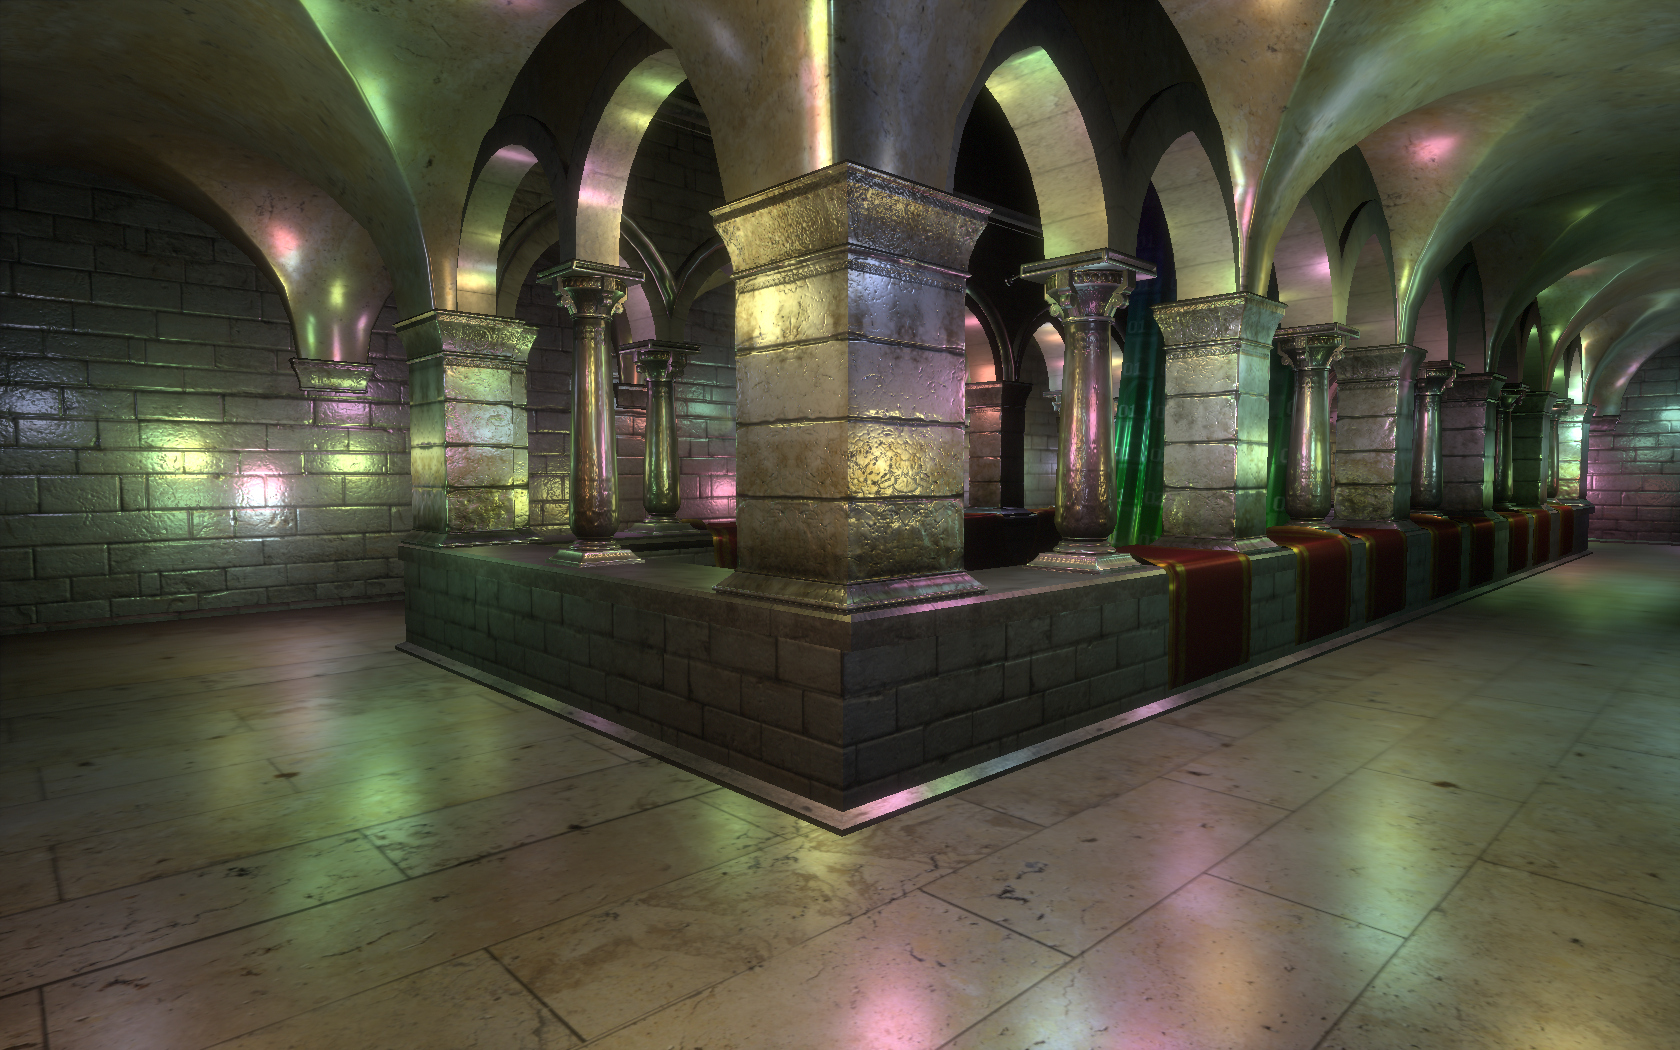
\includegraphics[width=0.9\linewidth]{./Figures/lightPrePass/sponza.jpg}
    \caption[Light pre-pass rendering of Sponza]{The ``Crytek Sponza'' scene under a complex lighting setup consisting of 100 spherical area lights using a custom convolution of the ABC reflectance model rendered via deferred lighting at 15 FPS at the 1680x1050 resolution.}
  \label{fig:lightPrePassSponza}
\end{figure}

\subsection{Geometry stage}

Most of the attributes required for the \emph{G-buffer} are computed by the \emph{Structure} kernel. Still, a \emph{Material} kernel may want to alter the normals in order to simulate a bumpy surface. These altered normals must be written into the \emph{G-buffer}. Hence, the first stage composes the two kernels and selectively writes their outputs to the \emph{G-buffer} as shown in Figure \ref{fig:DeferredLightingStage1}. The \emph{Material} kernel possibly writes more outputs than this stage uses, however, graph reduction is performed, so only the relevant parts are actually used at runtime. The \emph{Cg} compiler effectively removes any other extra computations.

\begin{figure}[h!]
  \centering
    \digraph[width=0.5\linewidth]{DeferredLightingStage1}{
	"Structure" -> "Material";
	"Material" -> "G-buffer";
    }
    \caption[Light Pre-Pass Stage 1]{The composition of kernels for the \emph{Geometry} stage of the  \emph{light pre-pass} rendering algorithm}
  \label{fig:DeferredLightingStage1}
\end{figure}

The \emph{G-buffer} has the following layout:

\begin{center}
\begin{tabular}{ | c | c | c | c | }
\hline
\multicolumn{4}{|c|}{ depth : f32 } \\
\hline
normal\_a:f16 & normal\_b:f16 & surface\_id:f16 & roughness:f16 \\
\hline
\end{tabular}
\end{center}

The normalized view-space normal is encoded in the \emph{G-buffer} using the \emph{Lambert Azimuthal Equal-Area projection} \cite{ArasNormalStorage}.

\subsection{Light stage}

Deferred renderers are notorious for being quite rigid with respect to illumination models achievable with them. This is because once the G-buffer is rendered, the light stage doesn't have access to per-object shaders, which might perform custom shading. Light volumes must then be rendered with the same shader for each pixel, regardless of which scene object a fragment in the G-buffer comes from.

A common approach is to use just one reflectance model ( usually the half-angle version of Phong's ) for all pixels and only control roughness. This may work just fine for games which don't require drastically varying surface styles.

Another solution is to render the majority of the scene using deferred rendering, but fall-back to forward rendering for surfaces requiring a different reflection model. Such an approach means that objects using the second-class reflectance models have to be used sparingly, and thus form a constraint imposed on artists.

The approach which Nucleus takes instead is not a novel one, but hasn't been widely adopted due to being costly on past generations of graphics hardware.

The G-buffer stores the \emph{surface ID} to be used at a given pixel and a fragment shader of the light stage branches on it, choosing the appropriate \emph{Reflectance} kernel implementation. The kernel index and parameters for it are stored in a texture, into which the \emph{G-buffer} contains a coordinate. The current approach allows up to 256 different surfaces, each of which might potentially use a different \emph{Reflectance} kernel. Obviously, this is not free either, however with the advent of real branching in recent GPU generations means that in practice the cost is not very high [TODO: numbers].

The code template used to compose multiple BRDFs together has the following structure:

\begin{lstlisting}[frame=single]
float surfaceId = tex2D(attribTex, uv);
float reflectanceId = tex2D(surfaceId, float2(surfaceId, 0));
 
if (reflectanceId < A) {
    result = BRDF1(
        tex2D(surfaceId, float2(surfaceId, ...)),
        tex2D(surfaceId, float2(surfaceId, ...)),
        tex2D(surfaceId, float2(surfaceId, ...))
    )
} else if (reflectanceId < B) {
    result = BRDF2(...);
} else if (reflectanceId < C) {
    ...
} else {
    ...
}
\end{lstlisting}

The code template includes dependent texture fetches and heavy branching. This is an obvious source of execution and memory fetch latency, however modern GPU architectures are able to hide some of it. [TODO: ref the latest Siggraph paper about GPU pipelines].
% TODO: move this to the future work section?
If this branching still turns out to be prohibitive, it's possible to reduce its cost using tile-based deferred rendering similar to [TODO: ref]. The framebuffer would be split into tiles, depending on whether they need the branch or not. Depending on the scene, many branches might use just a single BRDF, for which a specialized shader can be compiled.

As any of the other passes, the \emph{Light stage} generates a kernel graph (an example of which is shown in Figure \ref{fig:DeferredLightingStage2}), the only distinction is that it's compiled for the purpose of rendering the bounding volumes of lights.

\begin{figure}[h!]
  \centering
    \digraph[width=0.9\linewidth]{DeferredLightingStage2}{
	"G-buffer" -> "Reflectance1";
	"G-buffer" -> "Reflectance2";
	"G-buffer" -> "Reflectance3";
	"G-buffer" -> "Light";
	"Reflectance1" -> "switch";
	"Reflectance2" -> "switch";
	"Reflectance3" -> "switch";
	"switch" -> "Reflectance";
	"Light" -> "Reflectance";
	"Reflectance" -> "Illumination buffer";
    }
    \caption[Light Pre-Pass Stage 2]{The composition of kernels for the \emph{Light} stage of the  \emph{light pre-pass} rendering algorithm}
  \label{fig:DeferredLightingStage2}
\end{figure}

The current implementation uses a geometry shader to instantiate a cube for each light, taking a single point as the input. Only the quads facing away from the camera are drawn and reverse depth testing is performed in order to do approximate light culling. \\
Such setup will enable rendering of thousands of lights in a single batch, however this is not implemented yet. The downside of doing this for every light type would be large overdraw, since some lights may span a large portion of the screen and would benefit from more exact culling instead. Because of this, lights are actually drawn in separate batches, and approximate culling of their volumes is performed via the EXT\_depth\_bounds\_test OpenGL extension. Whereas the aforementioned reverse depth test allows culling of light volumes which are entirely in front of scene geometry, it doesn't do anything about the volumes being behind geometry. Depth bounds testing allows a range of depth values to be specified, so that no fragment is rendered if the value \emph{already in the depth buffer} is outside of this range. By conservatively specifying the minimum and maximum depth values of light volumes for this test, this effectively allows coarse culling. Figure \ref{fig:lightingComplexityComparison} demonstrates a case where the lighting complexity is reduced dramatically due to scene occlusion.

\begin{figure}[h!]
  \centering
  \subfigure[Reverse-Z]{\label{fig:lightingComplexity2}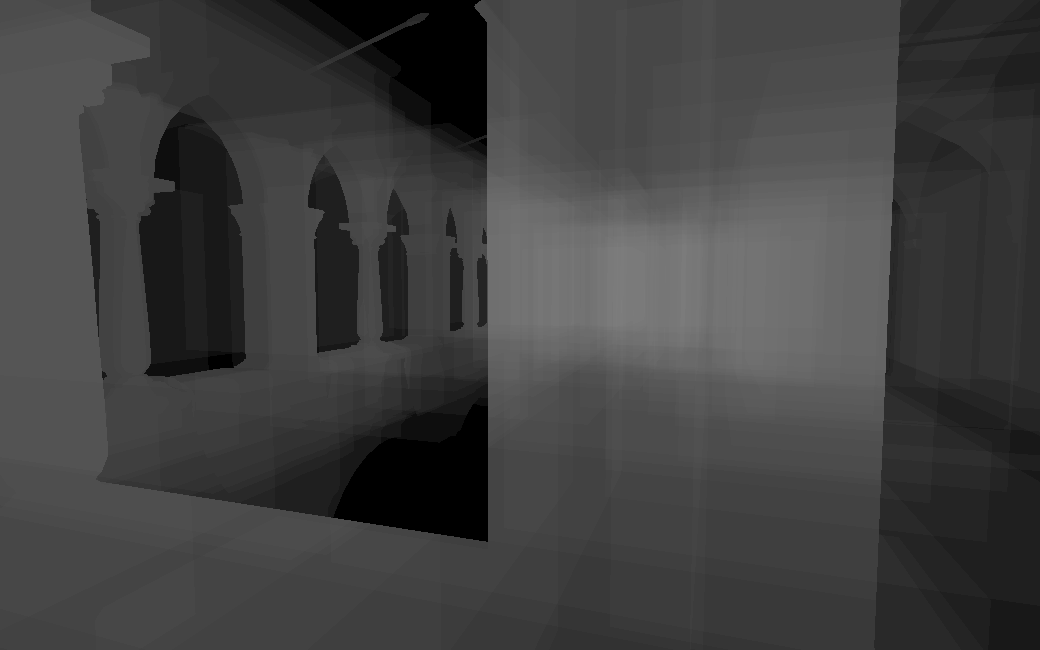
\includegraphics[width=0.45\linewidth]{./Figures/lightPrePass/lightingComplexity2.png}}
  \subfigure[Reverse-Z and bounds test]{\label{fig:lightingComplexity1}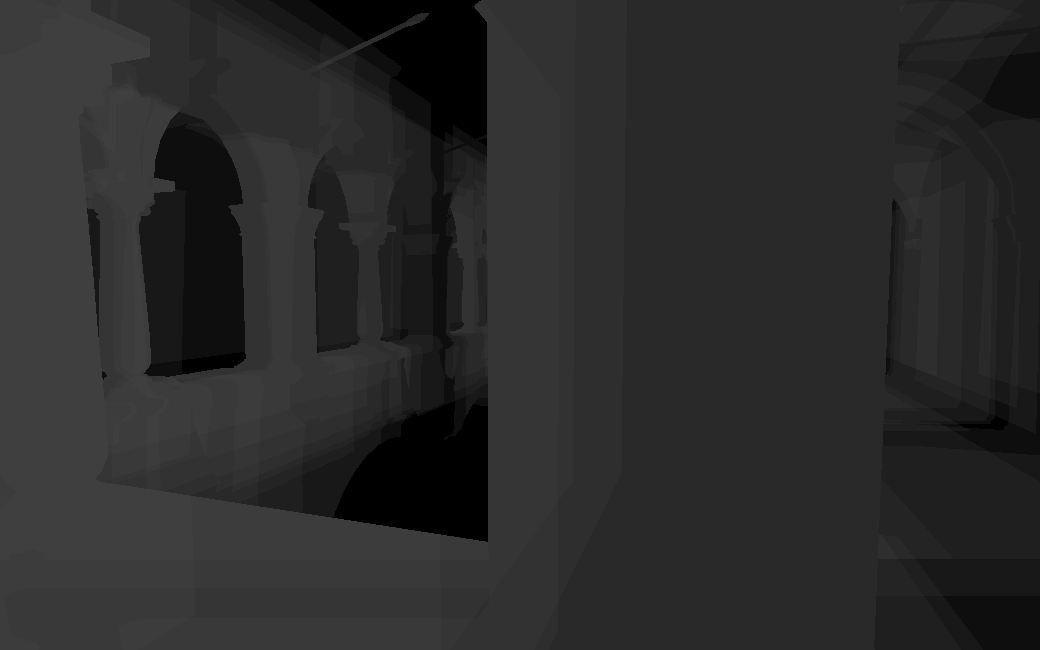
\includegraphics[width=0.45\linewidth]{./Figures/lightPrePass/lightingComplexity1.png}}
  \caption[Light volume culling comparison]{Comparison of lighting complexity with only reverse-Z culling and with bounds testing via EXT\_depth\_bounds\_test}
  \label{fig:lightingComplexityComparison}
\end{figure}

The illumination is rendered to a framebuffer of the same resolution as the screen, with two floating-point RGB attachments --- one for the diffuse illumination component, another for the specular.

\subsection{Light bounding}

It's not physically correct to constrain light falloff to a volume, since real lights don't have a limited range. Still, at a certain distance, the influence becomes negligible and of little use as an artistic tool, while still having the same computational overhead as at meaningful intensities. Therefore, the size of the bounding volume is calculated such that it cuts off at a certain distance, which depends on the intensity of the source. It's impractical to set the fade-out distance as far as to avoid a perceptual difference, therefore the size is calculated aggressively (the current implementation cuts off at 1\% the normalized intensity) and light falloff is modified to smoothly disappear into zero.

In physics, the intensity of light is inversely proportional to the squared distance from the source:
	
\[
	I = \frac{L}{r^2}
\]

where $L$ is a constant representing the luminous intensity of the light.

Whereas this law may be used in its exact form (and many implementations do), it is important to notice that it is valid only for idealized \emph{point} light sources. The intensity at distance close to zero quickly approaches infinity, resulting in rendering artifacts. Real world lights have a non-zero area which makes the falloff look different, especially close to the source. For this reason, the model
\[
	I = \frac{L}{1 + r^2}
\]
is sometimes used in computer graphics. It has the property of approaching $L$ near the source, making it easier to achieve a consistent appearance of objects under varying conditions. The default light falloff in Nucleus is therefore based on this model. It is then modified to fade out smoothly to $0$ in a limited range:
\[
	I = \frac{L * (1 - s(r^2 / r_m^2))}{1 + r^2}
\]
Where $r_m$ is the radius bounding the influence of the light and $s : float \rightarrow float$ is the Hermite interpolation function: \emph{smoothstep(0, 1, \_)} (an intrinsic in\emph{Cg} and \emph{HLSL}):
\[
	s(t) =
	\begin{cases}
	0 & t <= 0 \\
	1 & t >= 1 \\
	t^2 * (3 - 2t) & otherwise \\
	\end{cases}
\]

\begin{figure}[h!]
  \centering
  \subfigure[$1 / (1 + r^2)$ falloff]{\label{fig:lppInvSqFalloff1}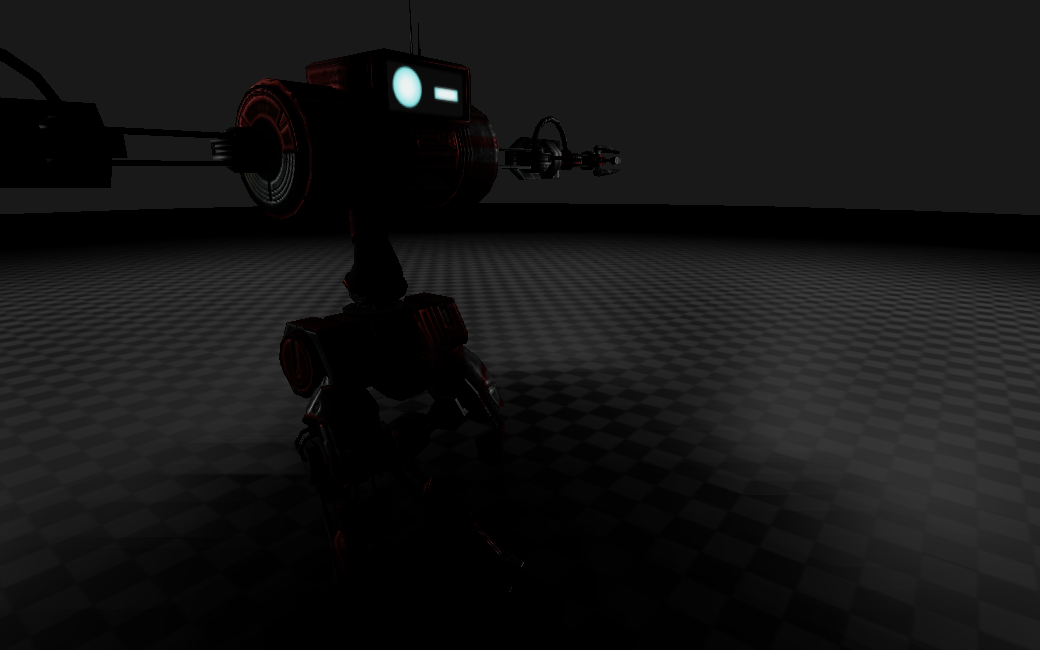
\includegraphics[width=0.45\linewidth]{./Figures/lightPrePass/invSq-1.png}}
  \subfigure[Modified $1 / (1 + r^2)$ falloff ]{\label{fig:lppModFalloff1}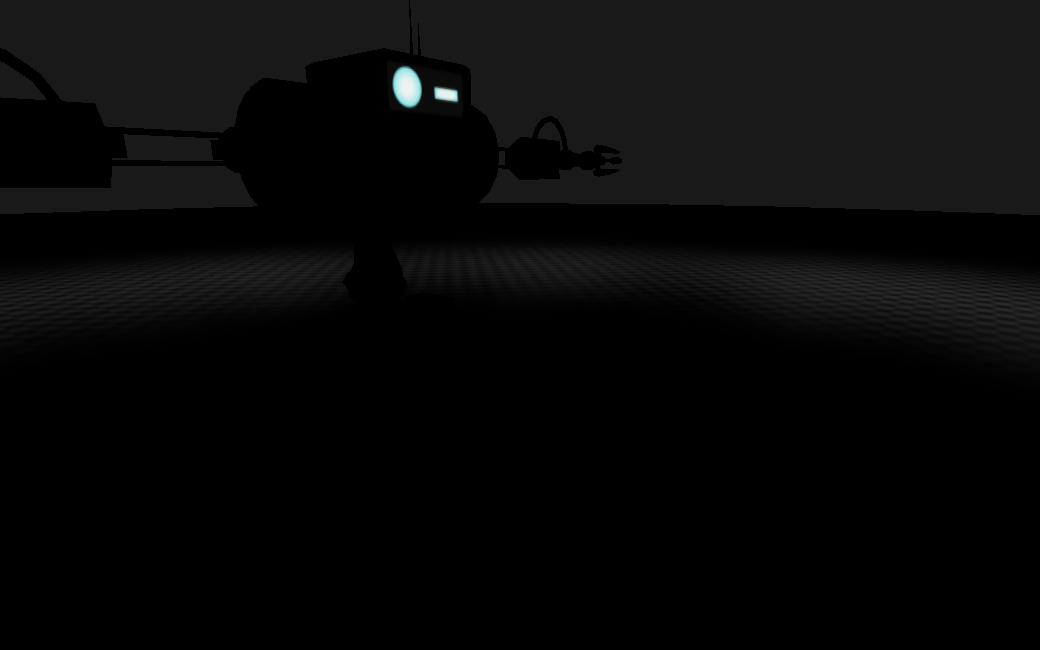
\includegraphics[width=0.45\linewidth]{./Figures/lightPrePass/mod-1.png}}
  \caption[Modified falloff, tricky case]{A tricky case for the modified light intensity falloff. ``UBot'' model courtesy of Eric Andrew.}
\label{fig:lppFalloffTrickyCase}
\end{figure}

\begin{figure}[h!]
  \centering
  \subfigure[$1 / (1 + r^2)$ falloff]{\label{fig:lppInvSqFalloff2}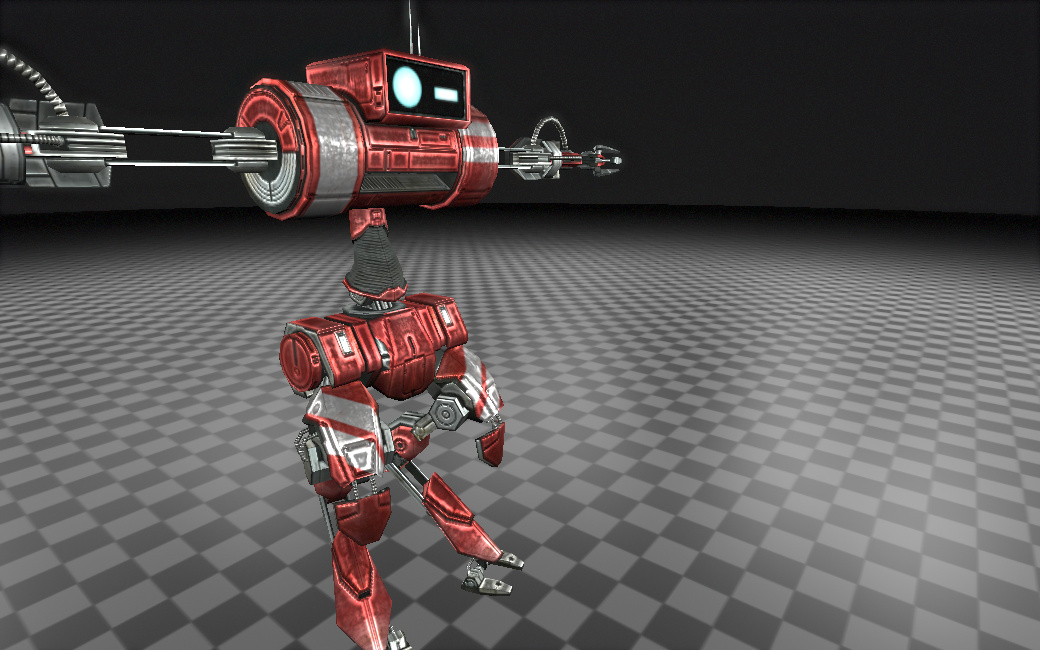
\includegraphics[width=0.45\linewidth]{./Figures/lightPrePass/invSq-2.jpg}}
  \subfigure[Modified $1 / (1 + r^2)$ falloff ]{\label{fig:lppModFalloff2}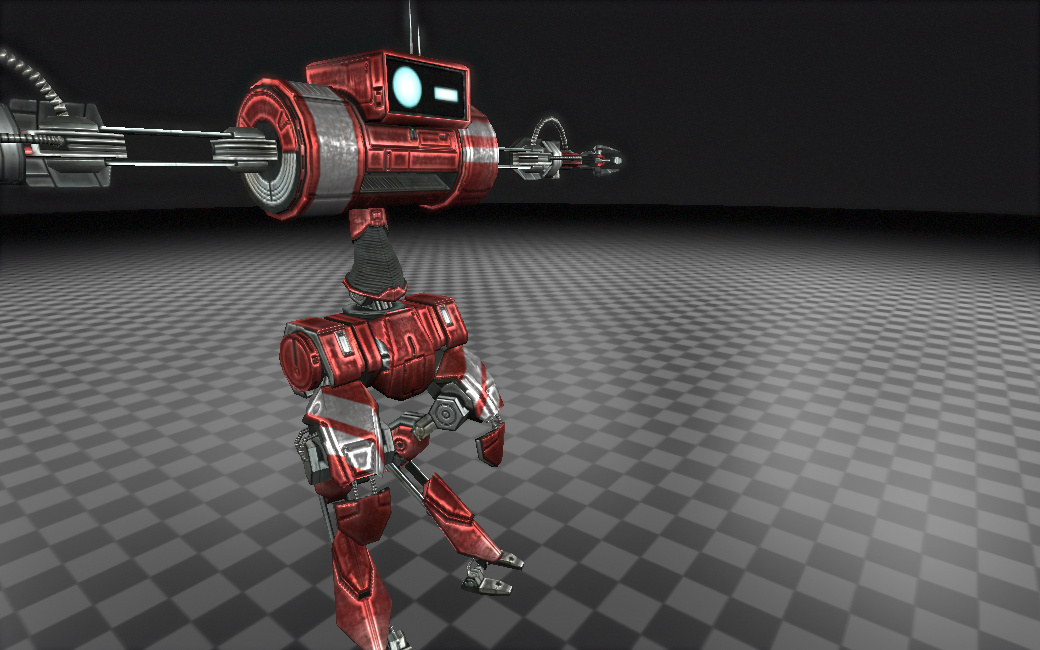
\includegraphics[width=0.45\linewidth]{./Figures/lightPrePass/mod-2.jpg}}
  \caption[Modified falloff, better case]{The modified falloff converging with $1 / (1 + r^2)$. ``UBot'' model courtesy of Eric Andrew.}
\label{fig:lppFalloffBetterCase}
\end{figure}

Figure \ref{fig:lppInvSqFalloff1} demonstrates the light clipping artifact when using inverse-square light falloff in the light pre-pass renderer -- the specular highlights are trimmed to the bounding cubes drawn around lights. Switching to the modified falloff model, we obtain figure \ref{fig:lppModFalloff1}. The clipping issue is gone, however the divergence between these models becomes very apparent. This is a particularly tricky case for the falloff, because the scene contains 200 very small, low-intensity lights. Increasing their yield and therefore the range used in the windowed model brings the two closer, as depicted in figure \ref{fig:lppFalloffBetterCase}. The divergence completely disappears under most normal lighting conditions. The scene configuration in figure \ref{fig:lppFalloffConverged} renders the same with either model, within the precision limits of the output image.

\begin{figure}[h!]
  \centering
    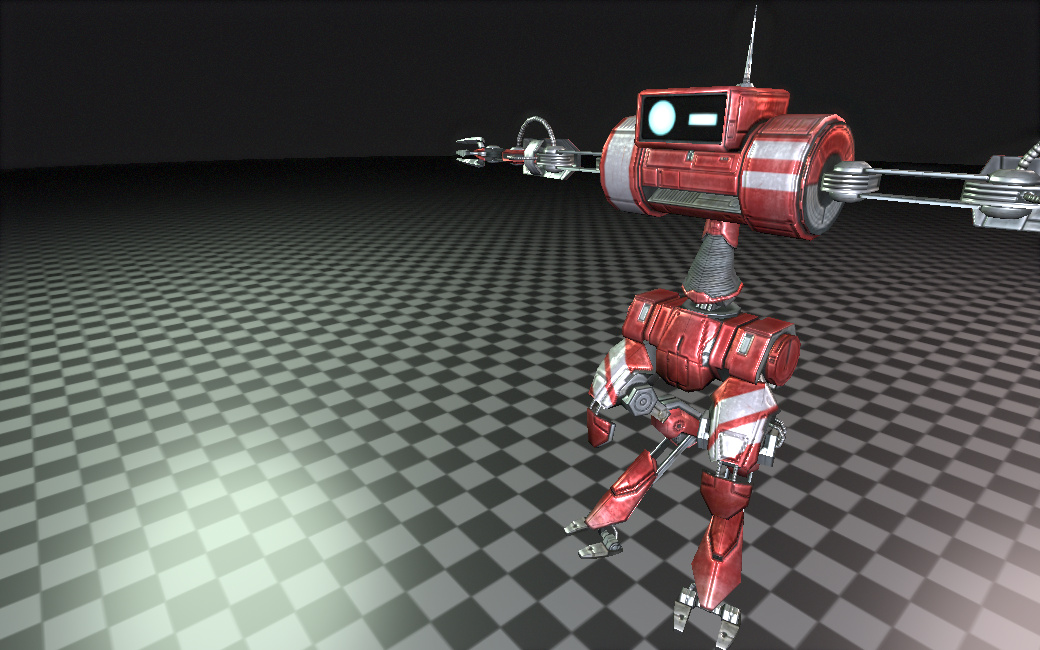
\includegraphics[width=0.45\linewidth]{./Figures/lightPrePass/falloffSame.jpg}
    \caption[Falloffs converged]{Both falloff models produce the same image. ``UBot'' model courtesy of Eric Andrew.}
  \label{fig:lppFalloffConverged}
\end{figure}

\subsection{Material stage}

Once the illumination buffer has been rendered, the final step is to combine it with scene object materials. In the light pre-pass algorithm, this is done by rendering the scene geometry again, in a similar fashion to regular forward rendering. The difference is that instead of computing the lighting, it's sampled from the previously rendered buffer. The diffuse part is multiplied by the material's albedo and the specular component -- by the specular tint of the material. The final radiance at the point is obtained by summing the two values.

\begin{figure}[h!]
  \centering
    \digraph[width=0.9\linewidth]{DeferredLightingStage3}{
    	"mul1" [
    		label = "*"
    	];
    	"mul2" [
    		label = "*"
    	];
	"Structure" -> "Material";
	"Diffuse illumination" -> "mul1";
	"Specular illumination" -> "mul2";
	"Material" -> "albedo";
	"albedo" -> "mul1";
	"Material" -> "specular tint";
	"specular tint" -> "mul2";
	"mul1" -> "+";
	"mul2" -> "+";
	"+" -> "output";
    }
    \caption[Light Pre-Pass Stage 3]{The composition of kernels for the \emph{Material} stage of the  \emph{light pre-pass} rendering algorithm}
  \label{fig:DeferredLightingStage3}
\end{figure}

\clearpage
\section{Shadows}

Shadows are an important part of 3-dimensional scene rendering. They provide visual cues relative object placement, help distinguish the shapes of objects and serve as a tool for mood shaping. Due to the direct integration of light sources which rasterization algorithms employ, shadows do not appear automatically, contrary to what might be expected from the rendering equation.

There are numerous ways of rendering shadows, however since in the context of this thesis they are only examples of using the rendering framework, I will not attempt to provide a survey of available methods. I will instead focus on \emph{shadow mapping}, a popular family of image-based algorithms offering a fine set of compromises for current hardware.

\subsection{A gentle introduction to standard shadow mapping}

Shadow mapping was first introduced by \citet{Williams78castingcurved} in 1978 and has since evolved into many similar algorithms. The following section contains a description of this standard algorithm, which is still in wide use due to its simplicity.

The core idea of shadow mapping is that of discretizing geometric information about a scene from the point of view of  light so that it may be quickly looked up when computing illumination during rendering. Assuming a point light, the task of determining whether a fragment is in shadow is equivalent to answering whether there is anything blocking a ray from this point to the position of the light. Standard shadow mapping allows this question to be answered quickly by querying an image containing distances to the nearest objects from the point of view of the light.

\begin{figure}[h!]
  \centering
  \subfigure[The A $<$ B shadowed fragment case]{\label{fig:ShadowMappingAlgorithmShadowed}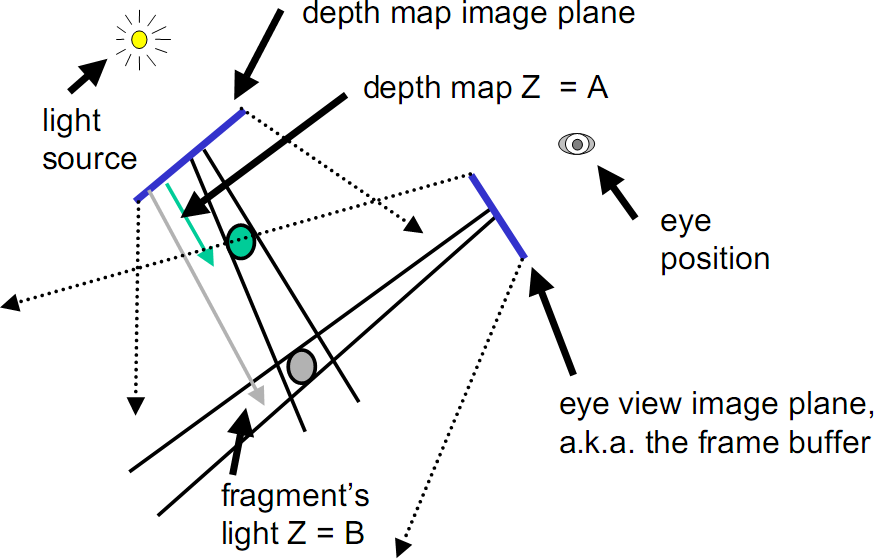
\includegraphics[width=0.45\linewidth]{./Figures/shadowMapping/shadowed.png}}
  \subfigure[The A $\cong$ B unshadowed fragment case]{\label{fig:ShadowMappingAlgorithmUnshadowed}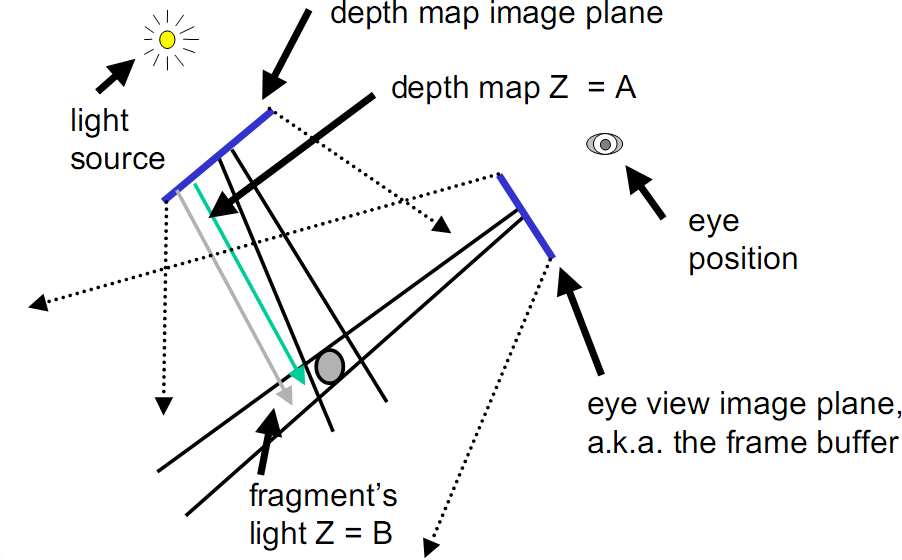
\includegraphics[width=0.45\linewidth]{./Figures/shadowMapping/unshadowed.png}}
  \caption{The shadow mapping algorithm. Images courtesy of Mark J. Kilgard, NVIDIA Corporation}
  \label{fig:ShadowMappingAlgorithm}
\end{figure}

Assuming that the light is a \emph{spot} with less than a 180$^\circ$ field of view, we can render an image containing distances to objects in the scene using regular rasterization and the \emph{depth-buffering} algorithm, which is very efficiently supported by graphics cards. The image contains distances to objects along rays starting at the light's position and traveling into the scene through positions of pixels in the virtual projection screen situated at the near clipping plane. The exact details to forming these rays are irrelevant here, the important detail is that they are effectively generated by the same perspective projection algorithm regular scene rendering uses. The resulting image is called a \textbf{depth map}.

During regular rendering, when a light's contribution to a fragment needs to be evaluated, this \emph{depth map} is used to approximately answer the visibility query. The fragment's world position is transformed via the same projection algorithm the depth map rendering used and as a result, a coordinate within the depth map is obtained. The pixel nearest to this coordinate contains the distance to the first object along the ray passing tho closest to the fragment out of all depth map samples. Comparing this stored value to the exact distance of the shaded fragment to the light (which is trivially calculable) answers the visibility test to within the precision of the depth map discretization. If the stored depth is smaller than the actual distance, the fragment is in shadow; otherwise, it is lit. In practice this comparison requires a slight bias due to the non-exact nature of the algorithm, but the core idea is just that.

TODO: more nice images

\subsection{Implementation of standard shadow mapping}

Most shadow mapping algorithms consist of two passes and the standard one is no exception. The first consists of rendering the shadow map, whereas the second pass ties into the evaluation of illumination when shading surfaces. The latter is a natural fit for implementing a custom \emph{light kernel}. The signature is:
	
\begin{lstlisting}[frame=single]
Light = kernel(
    in position <type float3 + use position + basis world>,
    out intensity <type float4 + use color>,
    out toLight <type float3 + basis world + use toLight>
);
\end{lstlisting}

The only output which will need to be calculated differently from regular, unshadowed rendering is \emph{intensity}. In order to compute it, the kernel will need information about the light instance in the first place. The \emph{position} parameter in the above kernel is only the position of the point being shaded, so all data for a light instance has to be defined within the implementation of the kernel.

\begin{figure}[h!]
  \centering
    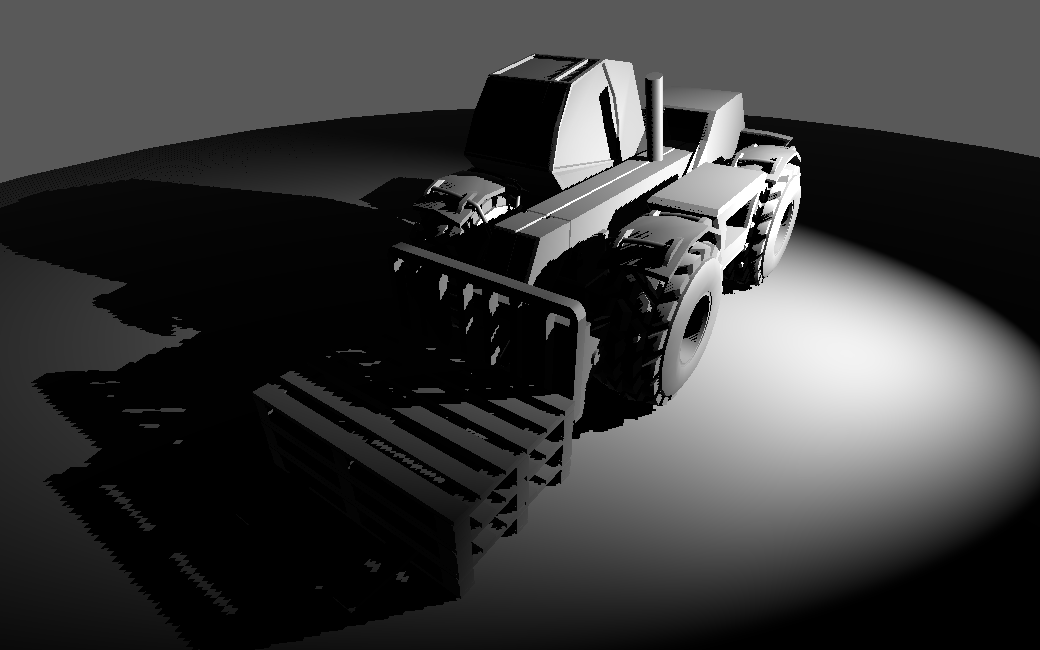
\includegraphics[width=0.9\linewidth]{./Figures/shadowMapping/manitouSM.png}
    \caption[SM in Nucleus]{Shadow Mapping in Nucleus. ``Manitou'' model courtesy of Marcin Banak.}
  \label{fig:NucleusSM}
\end{figure}

In section \ref{sec:Kernels}, it was mentioned that kernels can receive external data for their calculations. This is accomplished through \textbf{Data} graph nodes. These nodes provide \emph{uniform} parameters into the pipeline and their values need to be explicitly handled by an appropriate CPU-side entity associated with the particular kernel type. In case of \emph{light} kernels, these are \emph{Light} classes and instances of their sub-types. Besides preparing and binding attributes to kernels, these CPU-side entities allow easy manipulation of lights from the logical side of the application.

As for shadow map generation, the solution was mentioned in section \ref{sec:Renderers} and boils down to creating a custom \textbf{Renderer}. The implementation is much simpler than that of the \emph{forward} and \emph{light pre-pass} algorithms, because it only uses \emph{structure} kernels associated with \emph{renderables}. Since \emph{structure} kernels must output final positions of the geometry, they need only be connected to a simple kernel which calculates distances from the light.

Finally, this specialized \textbf{DepthRenderer} is used in a custom \textbf{SpotLight\_SM} class on the CPU side, which in turn is a façade for a GPU kernel of the same name. Figure (TODO) demonstrates this relationship.

Upon rendering a scene, the set of visible lights is determined and each \emph{Light} sub-class instance is given a chance to prepare data for the GPU phase of rendering. This is where instances of the custom class will perform depth map rendering.

\subsection{Variance shadow mapping}

One major drawbacks of standard shadow mapping is that depth maps cannot be filtered in the same way as color textures. This typically leads to severe aliasing. Filtering methods based on sampling the depth map multiple times per a shaded fragment, computing the visibility query and averaging the result provide acceptable results, but at a heavy price (TODO: ref Advanced Soft Shadow Mapping Techniques - NVIDIA).

\begin{figure}[h!]
  \centering
    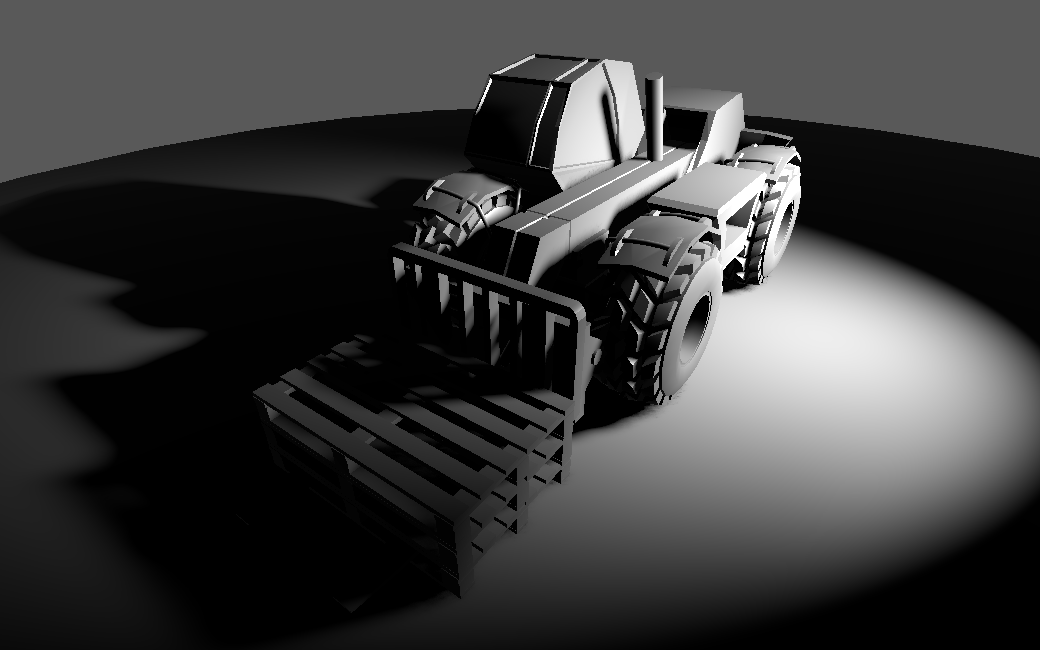
\includegraphics[width=0.9\linewidth]{./Figures/shadowMapping/manitouVSM.png}
    \caption[VSM in Nucleus]{Variance Shadow Mapping in Nucleus. ``Manitou'' model courtesy of Marcin Banak.}
  \label{fig:NucleusVSM}
\end{figure}

\citet{Donnelly06varianceshadow} present an interesting algorithm, which is simple to implement and solves the aliasing problem with low additional storage and computation. In the first step, it proceeds similarly to regular shadow mapping, but in addition to rendering the depths as seen form a light source, squares of the depth values are stored as well, hence rendering a two-component texture. The resulting texture can be filtered through the use of mipmapping, summed area tables and further softened by blurring.

The filtered texture is used to recover the moments $M_1$ and $M_2$ of a probabilistic distribution of depths around the filter region at any point within the image:
\begin{align*}
M_1 = E(x) &= \int_{-\infty}^\infty xp(x)dx \\
M_2 = E(x^2) &= \int_{-\infty}^\infty x^2p(x)dx
\end{align*}
From these, the mean $\mu$ and variance $\sigma^2$ are calculated:
\begin{align*}
\mu &= E(x) = M_1\\
\sigma^2 &= E(x^2) - E(x)^2 = M_2 - M_1^2
\end{align*}

Finally, we can compute the upper bound on the fraction of pixels within the filter region which are farther from the light source than a fixed depth $t$ using \emph{Chebychev's inequality}:
\[
P(X \geq t) \leq \frac{\sigma^2}{\sigma^2 + (t - \mu)^2} \;\;\;\; t < \mu
\]
where $X$ is a random variable drawn from a distribution with mean $\mu$ and variance $\sigma$.

When computing shadowing for a fragment seen from the camera, $t$ is the distance of the fragment from the light source and $P(X \geq t)$ gives an approximation of the fragment's visibility. For the case where $t \leq \mu$, it is assumed that the fragment is completely visible.

The algorithm has been implemented within Nucleus by creating a new light type and an associated kernel. In addition to rendering the moments map, the CPU side of the light implementation exploits the post-processing pipeline in order to perform separable Gaussian blurring of the texture. The implementation also uses light bleeding reduction by darkening the shadow as to perceptually improve on the upper bound given by Chebychev's inequality \cite{SATVSM}.

\clearpage
\section{Post-processing effects}

Several post-processing effects were implemented in order to test the pipeline. Figure \ref{fig:postProcOff} shows a test scene. The high-dynamic range output of this rendering is supplied to a \emph{PostProcessor} before gamma-correction. The image is mapped onto a full-screen quadrilateral, which is rendered with shaders generated from a kernel graph.

\begin{figure}[h!]
  \centering
  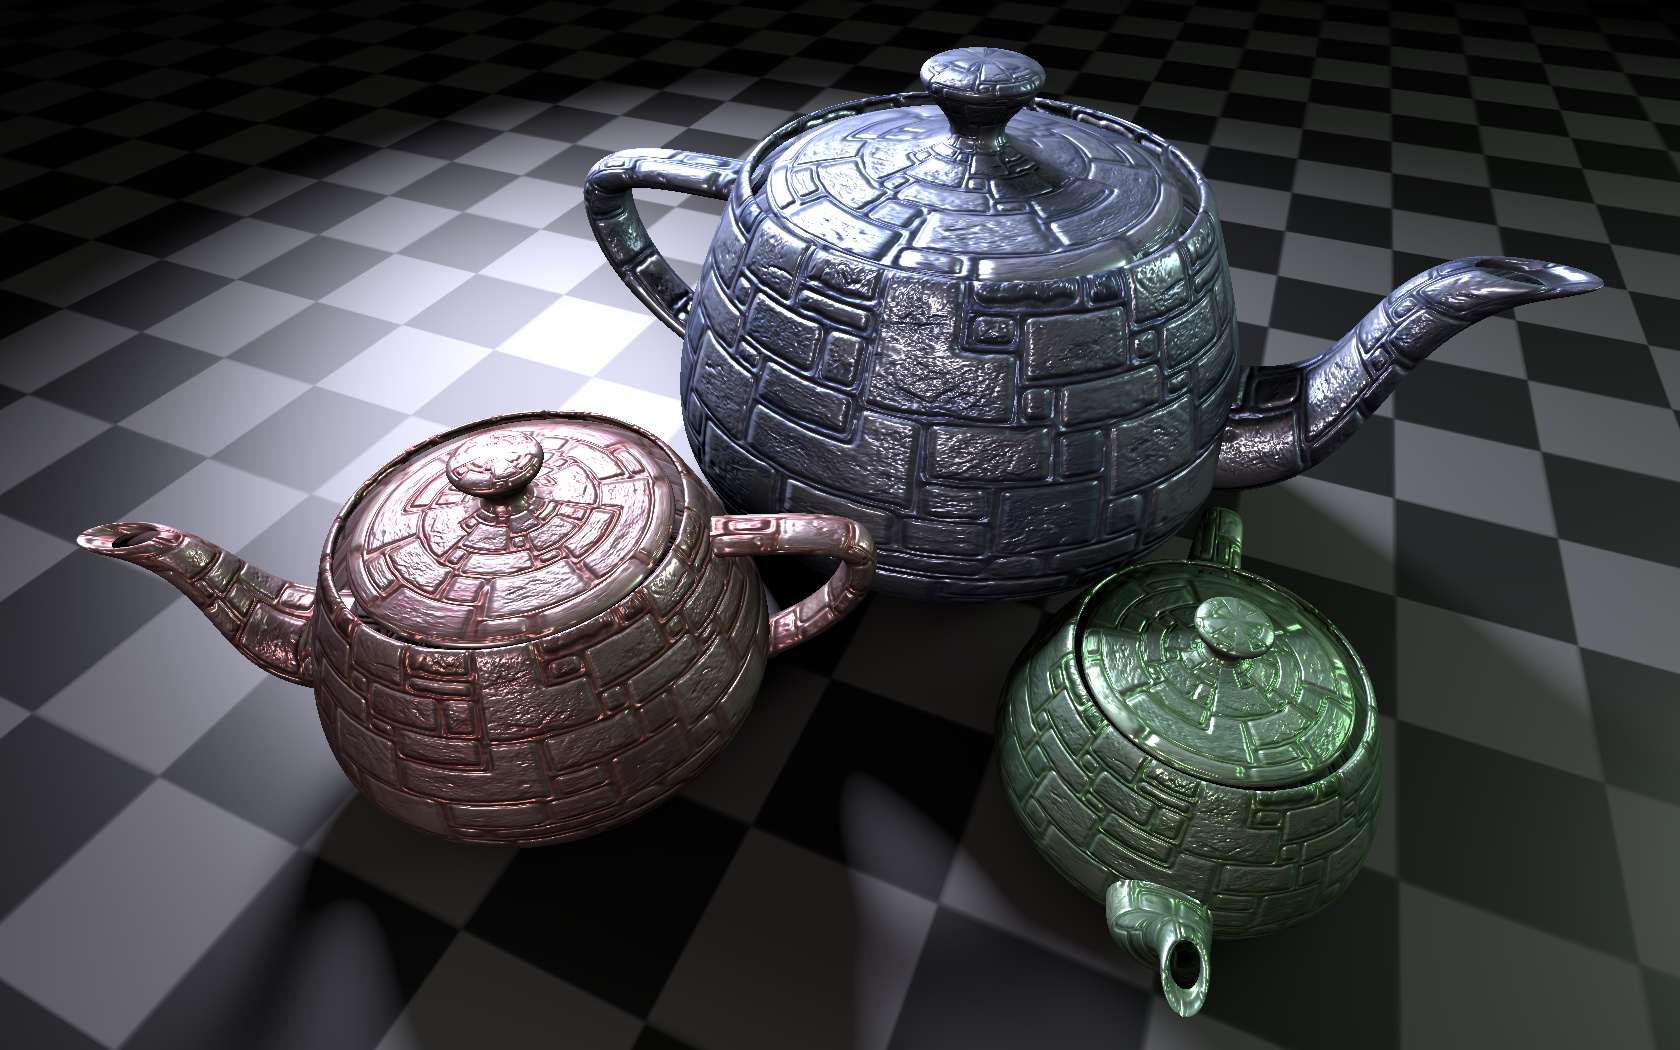
\includegraphics[width=0.45\linewidth]{./Figures/postProc/off.jpg}
  \caption[Post-processing test scene]{The scene used to test post-processing filters}
  \label{fig:postProcOff}
\end{figure}

\subsection{Uniform filters}

The most basic post-processing filters are ones which operate uniformly on individual samples without taking any other parts of the image into consideration. Figure \ref{fig:postProcSimple} demonstrates two such filters. They are implemented as simple \emph{Cg} functions operating on individual colors, then automatically lifted to work on whole images by the functional composition mechanism described in section \ref{sec:FunctionalComposition}.

\begin{figure}[h!]
  \centering
  \subfigure[Negative]{\label{fig:postProcNegative}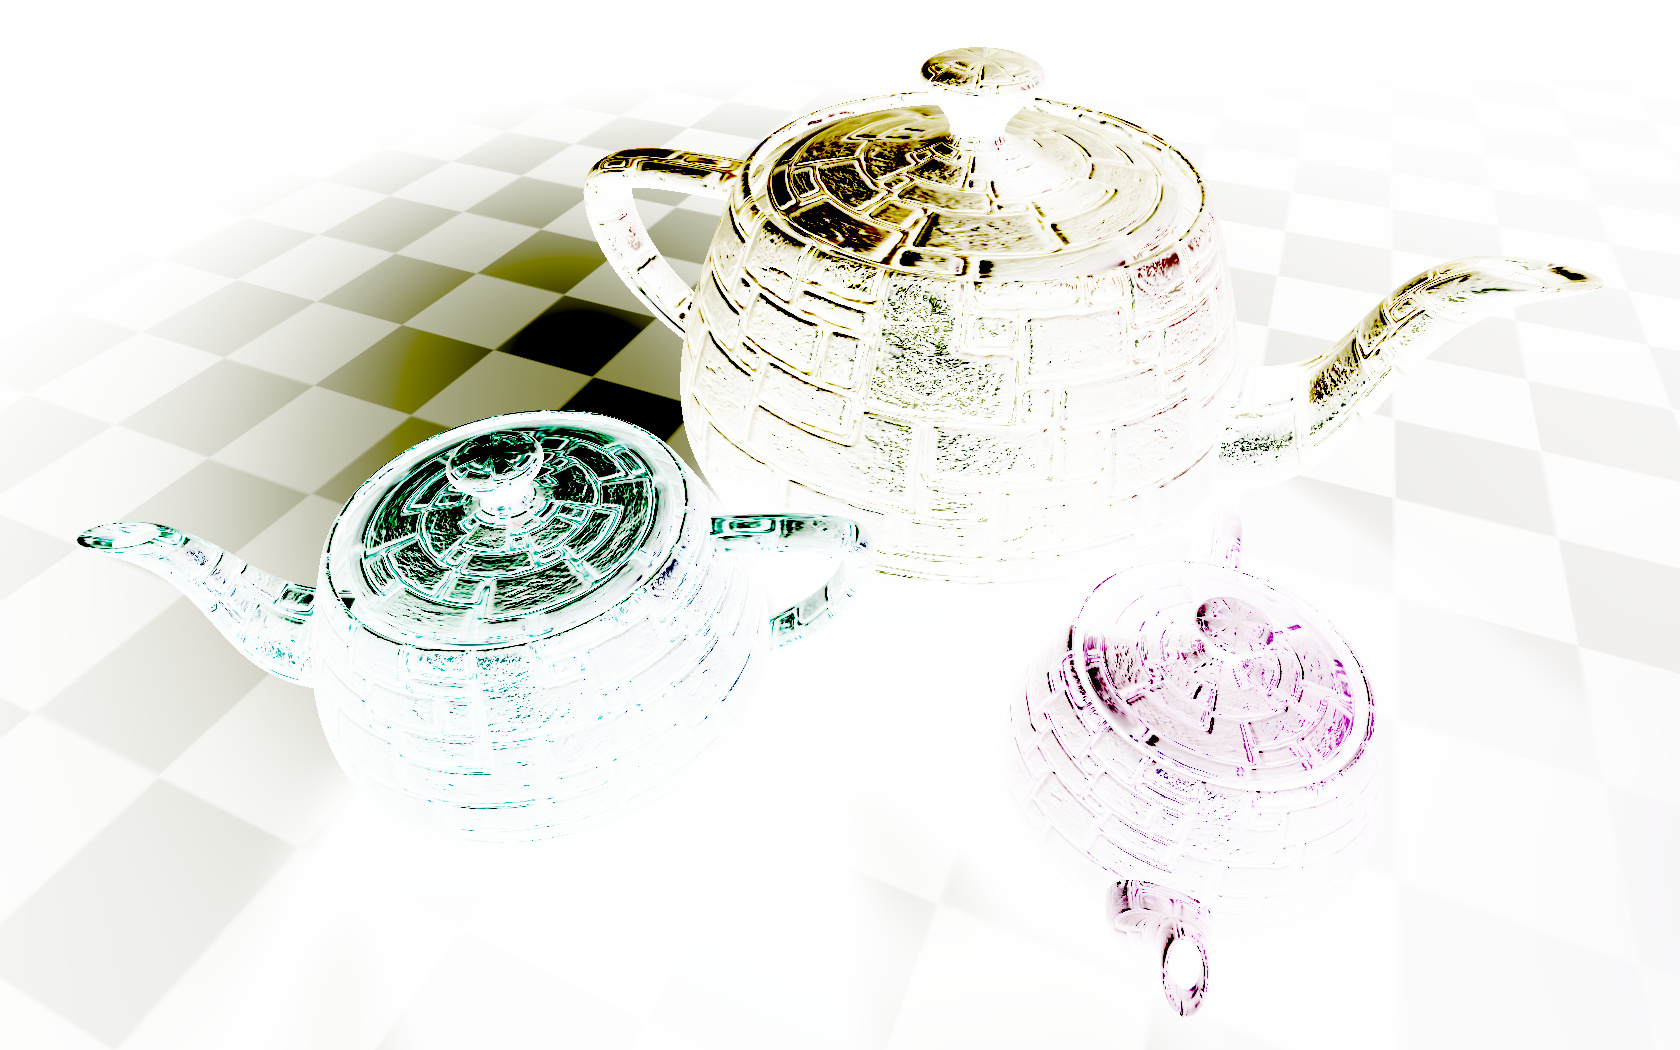
\includegraphics[width=0.45\linewidth]{./Figures/postProc/negative.jpg}}
  \subfigure[Desaturation]{\label{fig:postProcDesaturate}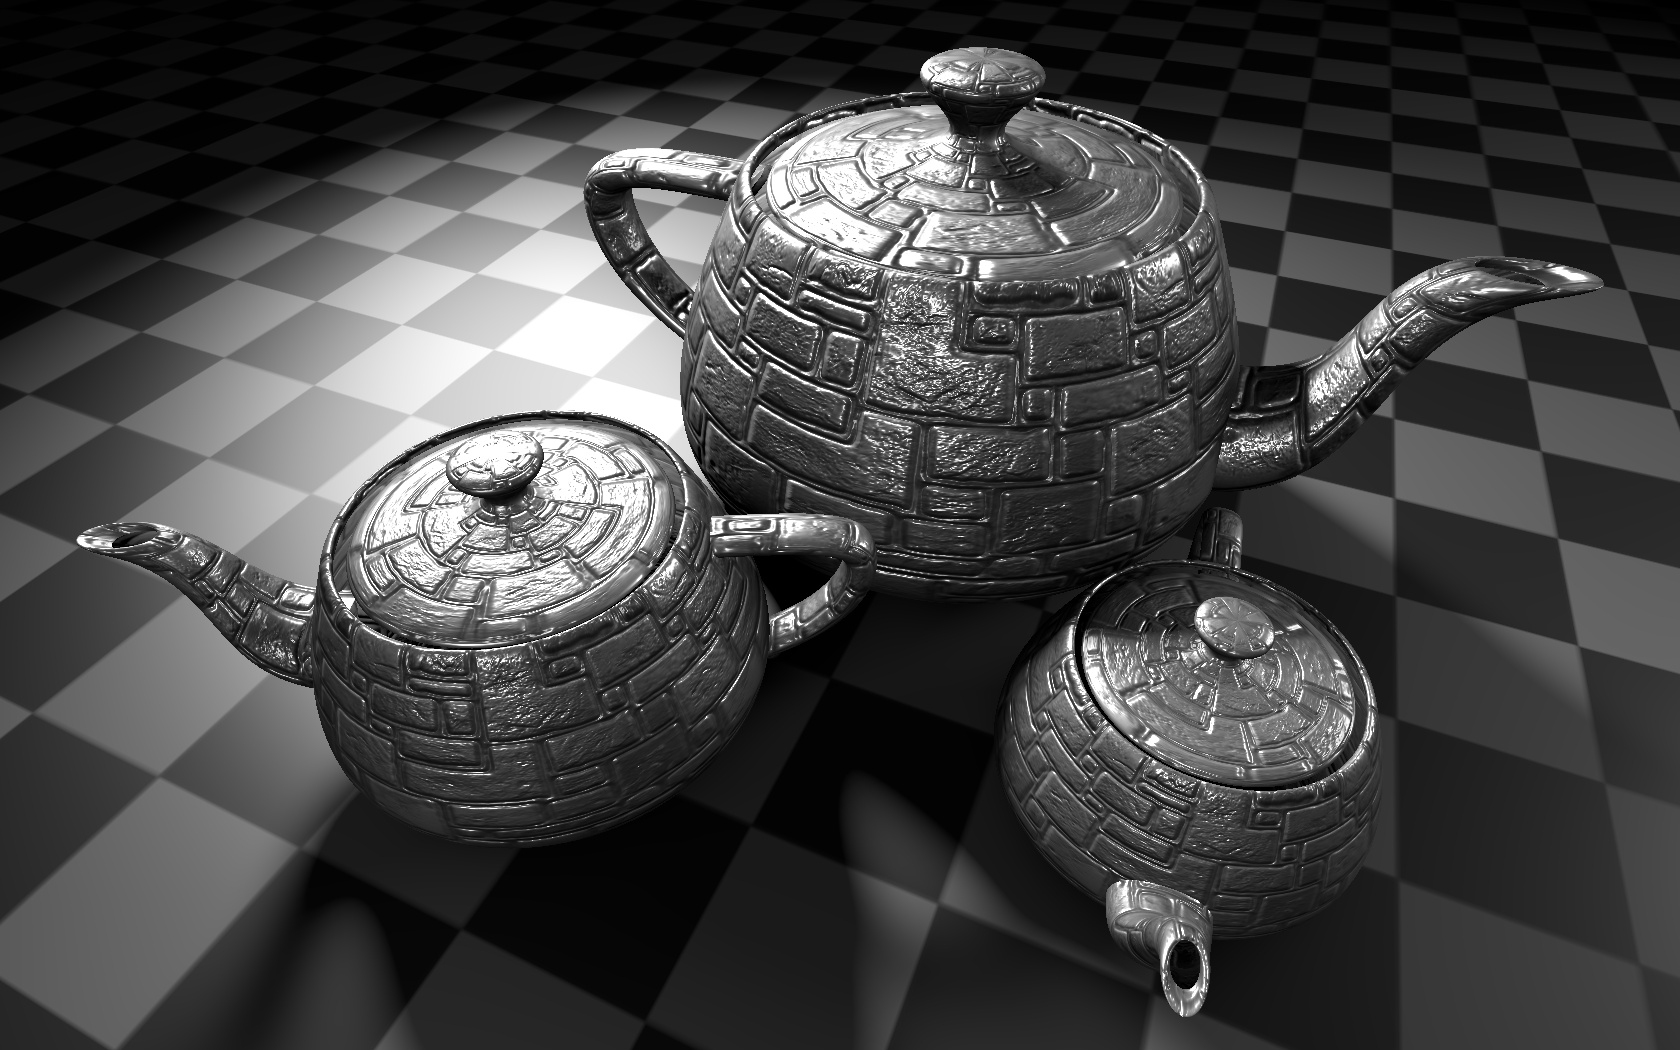
\includegraphics[width=0.45\linewidth]{./Figures/postProc/desaturation.jpg}}
  \caption{Simple uniform filters}
  \label{fig:postProcSimple}
\end{figure}

\subsection{Blur}

As mentioned in section \ref{sec:PostProcessing}, the post-processing system allows multi-pass rendering. One common application of this feature is computation of separable filters, such as the Gaussian blur shown in figure \ref{fig:postProcBlur}. The first image shows the result of convolving the signal with only a horizontal Gaussian kernel. A \emph{Blit} node is inserted after this step and followed by vertical blurring. This effectively approximates a complete two-dimensional Gaussian blur, however with an order of magnitude less samples taken from the image.

\begin{figure}[h!]
  \centering
  \subfigure[Horizontal]{\label{fig:postProcBlurHoriz}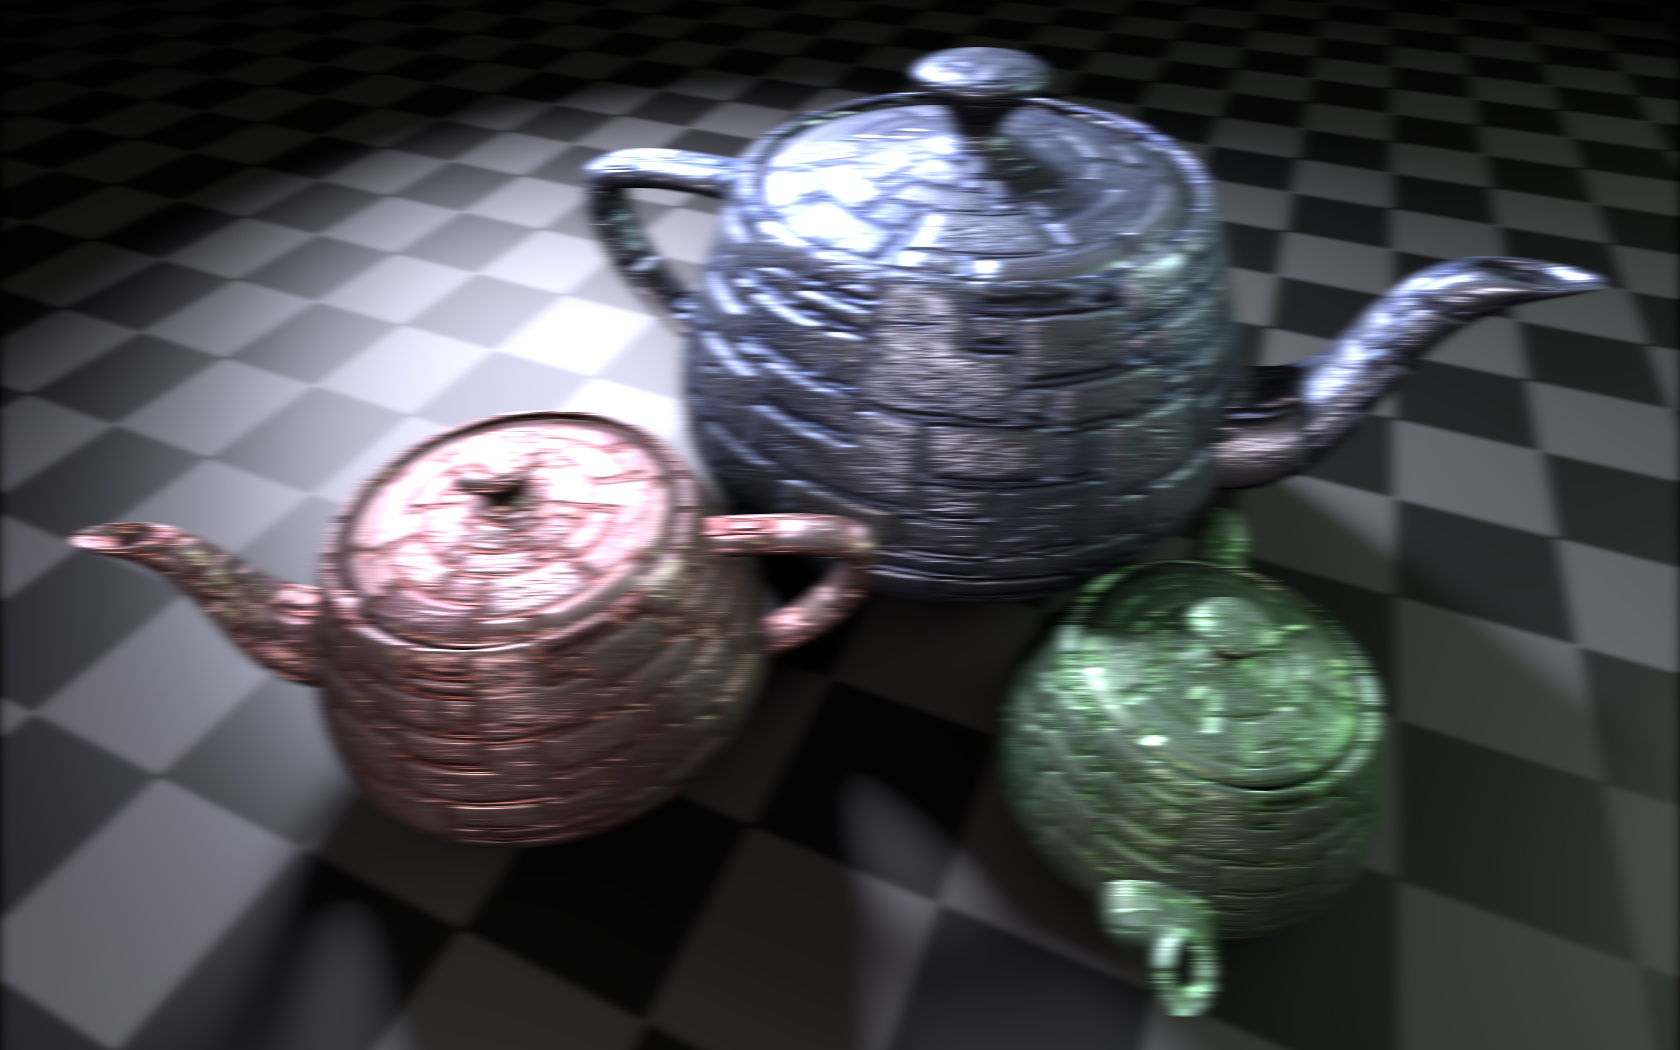
\includegraphics[width=0.45\linewidth]{./Figures/postProc/blurMoreHoriz.jpg}}
  \subfigure[Horizontal and vertical]{\label{fig:postProcBlurFull}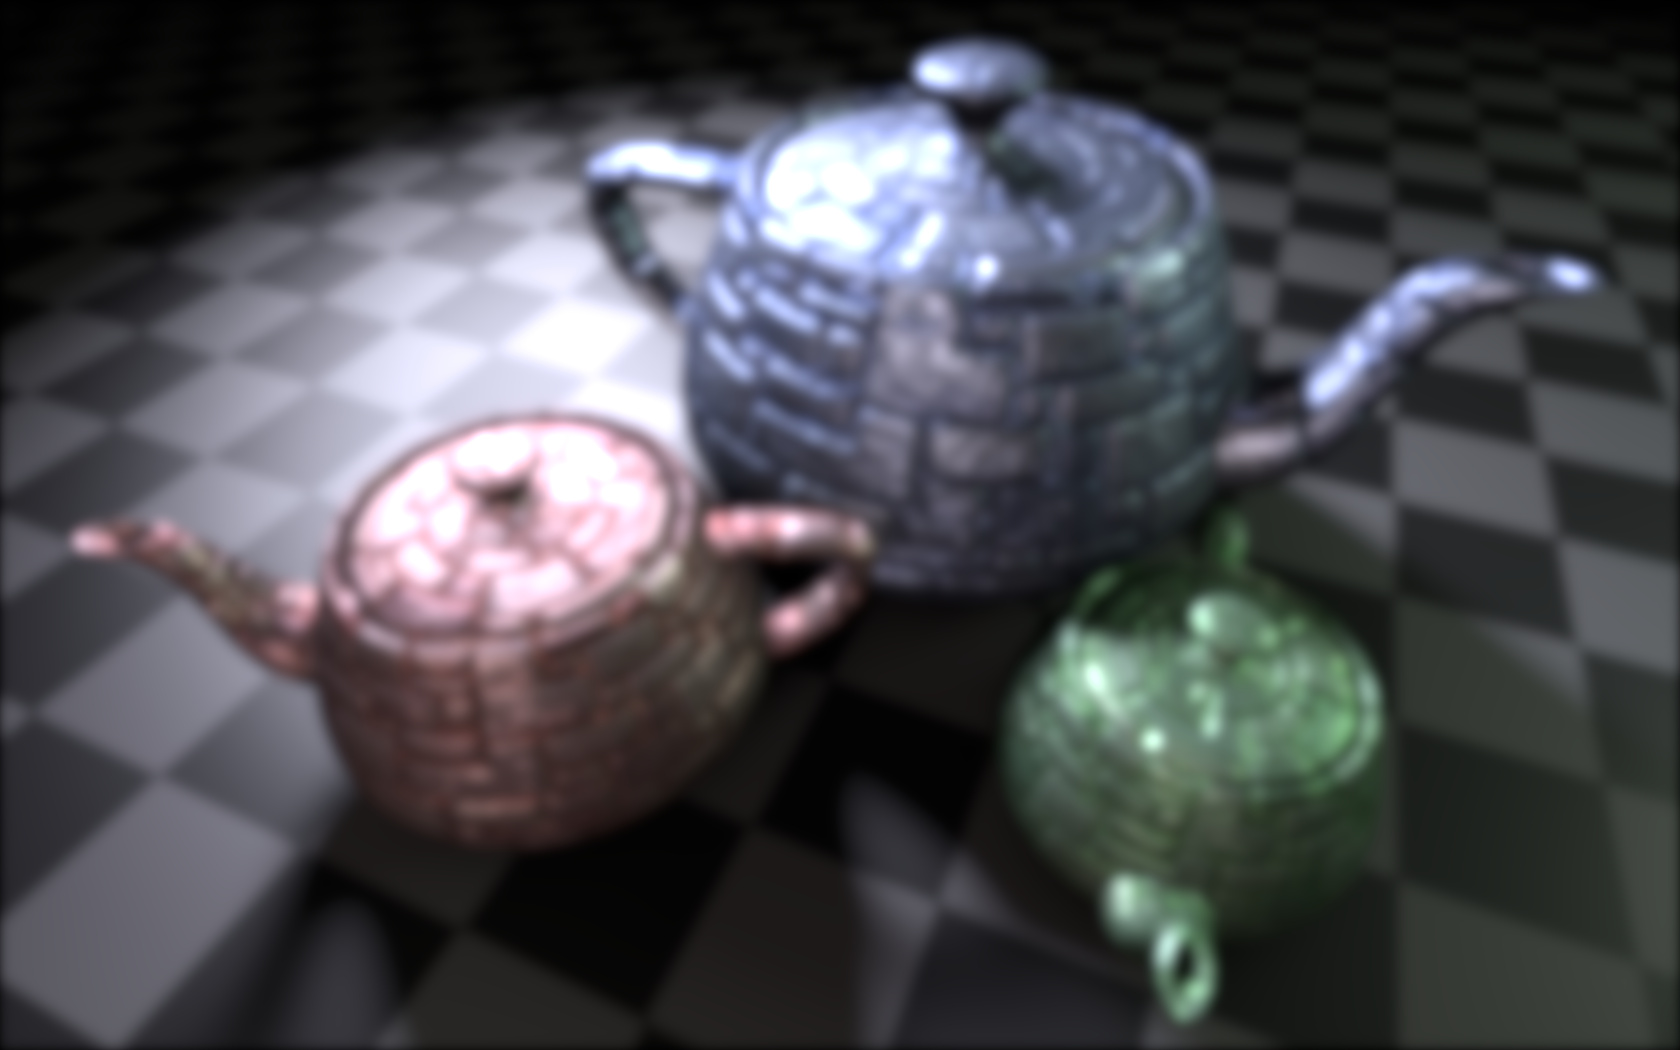
\includegraphics[width=0.45\linewidth]{./Figures/postProc/blurMore.jpg}}
  \caption{Gaussian blur}
  \label{fig:postProcBlur}
\end{figure}

\subsection{Glare}

A glare effect can improve the realism of a computer-generated image by simulating the effects which happen in the human visual systems at luminance values unattainable by current mainstream display technology \cite{Spencer95physicallybasedglare}. Consumer--level display devices are limited to 256--1024 luminance levels and max brightness levels of about 500 $cd/m^2$. For comparison, the clear daytime sky at horizon has about 10,000 $cd/m^2$ and fairly bright moonlight 0.01 $cd/m^2$ \cite{radiometryPhotometry}. There is simply no way to display such a varying range on a display device, therefore many effects responsible for realistic perception of the scene do not have a chance to form.

One of the sources of glare is light scattering within the cornea and the lens of the eye. \citet{Spencer95physicallybasedglare} note that it can be approximated with a sum of Gaussian-filtered images. The particular shape of this scattering effect varies from individual to individual, and while it may be evaluated experimentally and averaged, it is also an important artistic tool.

The example glare filter implemented within Nucleus uses a combination of four hierarchically blurred images, weighted by empirically obtained values and summed with the original image. Figure \ref{fig:postProcGlare} demonstrates an exaggerated version of this post-processing effect.

\begin{figure}[h!]
  \centering
    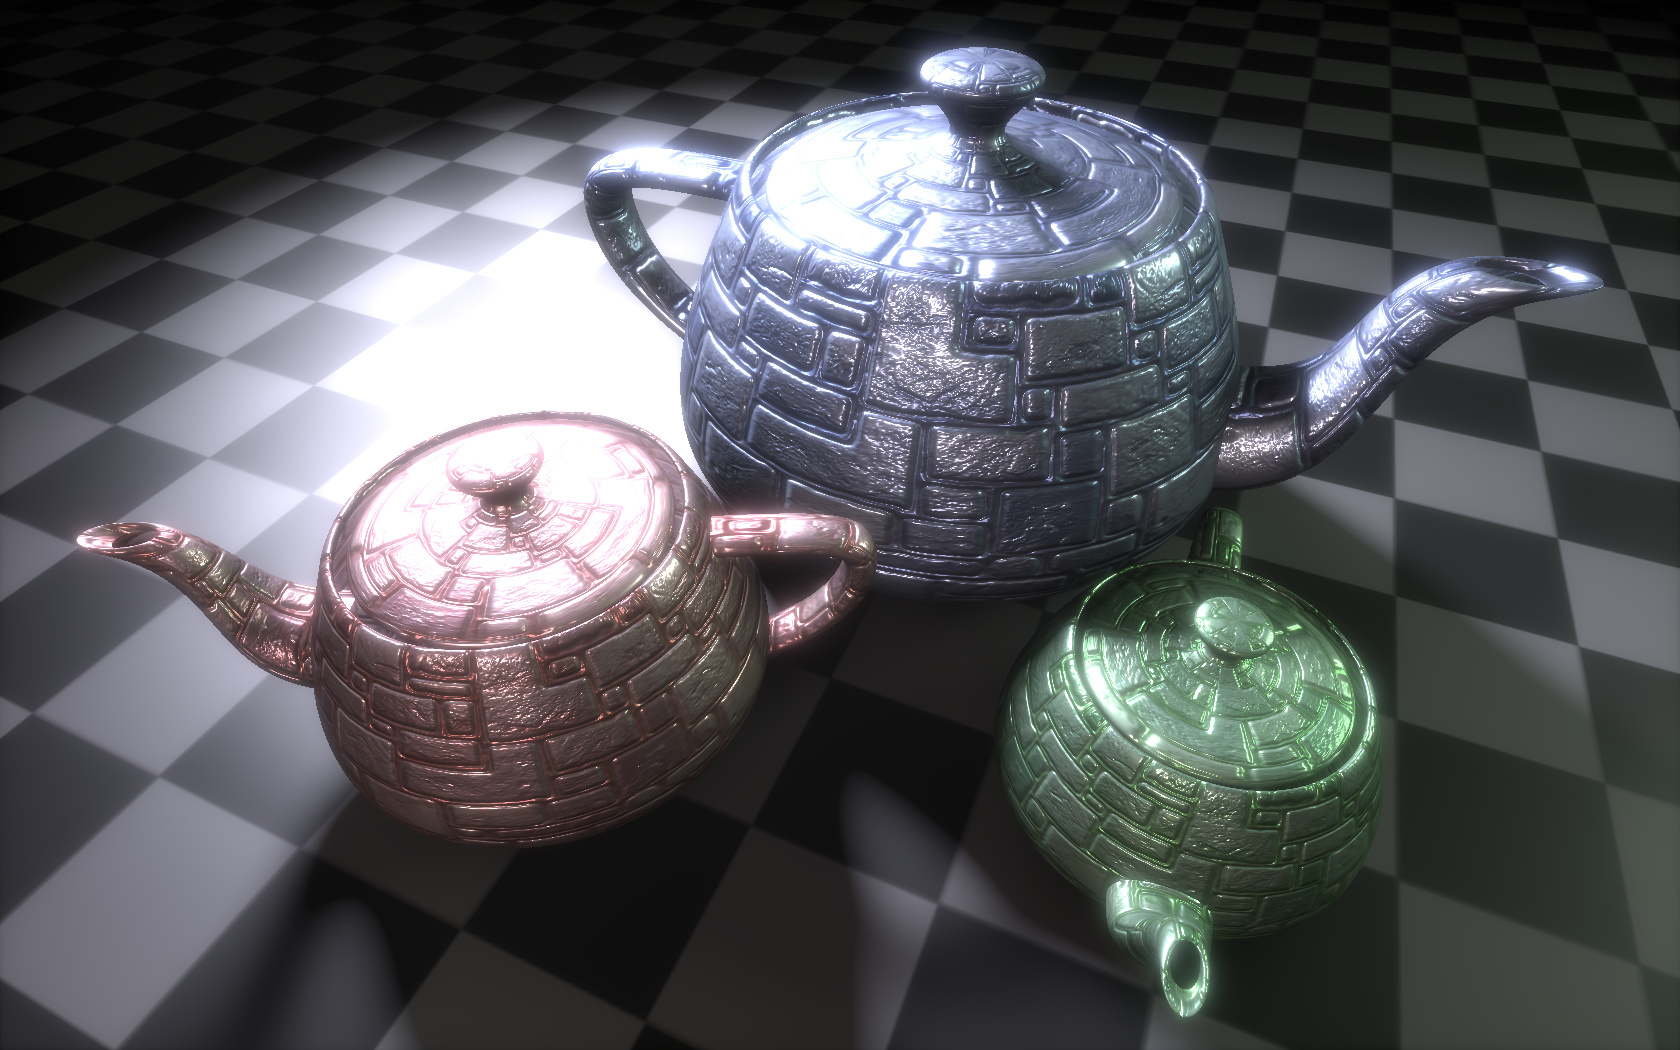
\includegraphics[width=0.9\linewidth]{./Figures/postProc/glare.jpg}
    \caption[Glare]{Multi-scale glare applied to the test scene (exaggerated)}
  \label{fig:postProcGlare}
\end{figure}

\subsection{Spatial acuity and color sensitivity reduction}

Simulations of some form of glare are common in real-time rendering systems -- most commonly known as ``bloom'', they actually aim to simulate camera lens. However, besides glare, which is mostly apparent in high contrast situations, the human visual system exhibits another phenomenon, which unfortunately is rarely tackled by computer graphics. Under low luminance conditions, \emph{cone cells} in the eye are mostly nonfunctional. Because cone cells are the component of the human visual system which allows us to perceive colors, lack of their activation means that in low luminance conditions, human vision is monochromatic, perceived with a slight blue tint. Additionally, experimental subjects often describe this ``scotopic vision'' as blurry and noisy \cite{Thompson_aspatial}.

\citet{Thompson_aspatial} have proposed an empirically-based low-luminance post-processing filter. Since it uses images convolved by Gaussian kernels, it comes at a slight additional cost to glare simulation -- in fact, the two filters have been merged into one within Nucleus. The post-processing kernel first computes an acuity value (figure \ref{fig:postProcAcuityMap}) for each pixel of the processed image, then uses this value to interpolate between the regular color (photopic vision) and the result of the scotopic filter. The acuity value is calculated by passing samples of the blurred images through a step function, then blending them together using the ``screen'' method ($1 - (1-a)*(1-b)$).

\begin{figure}[h!]
  \centering
  \subfigure[Post-processing off]{\label{fig:postProcNoAcuity}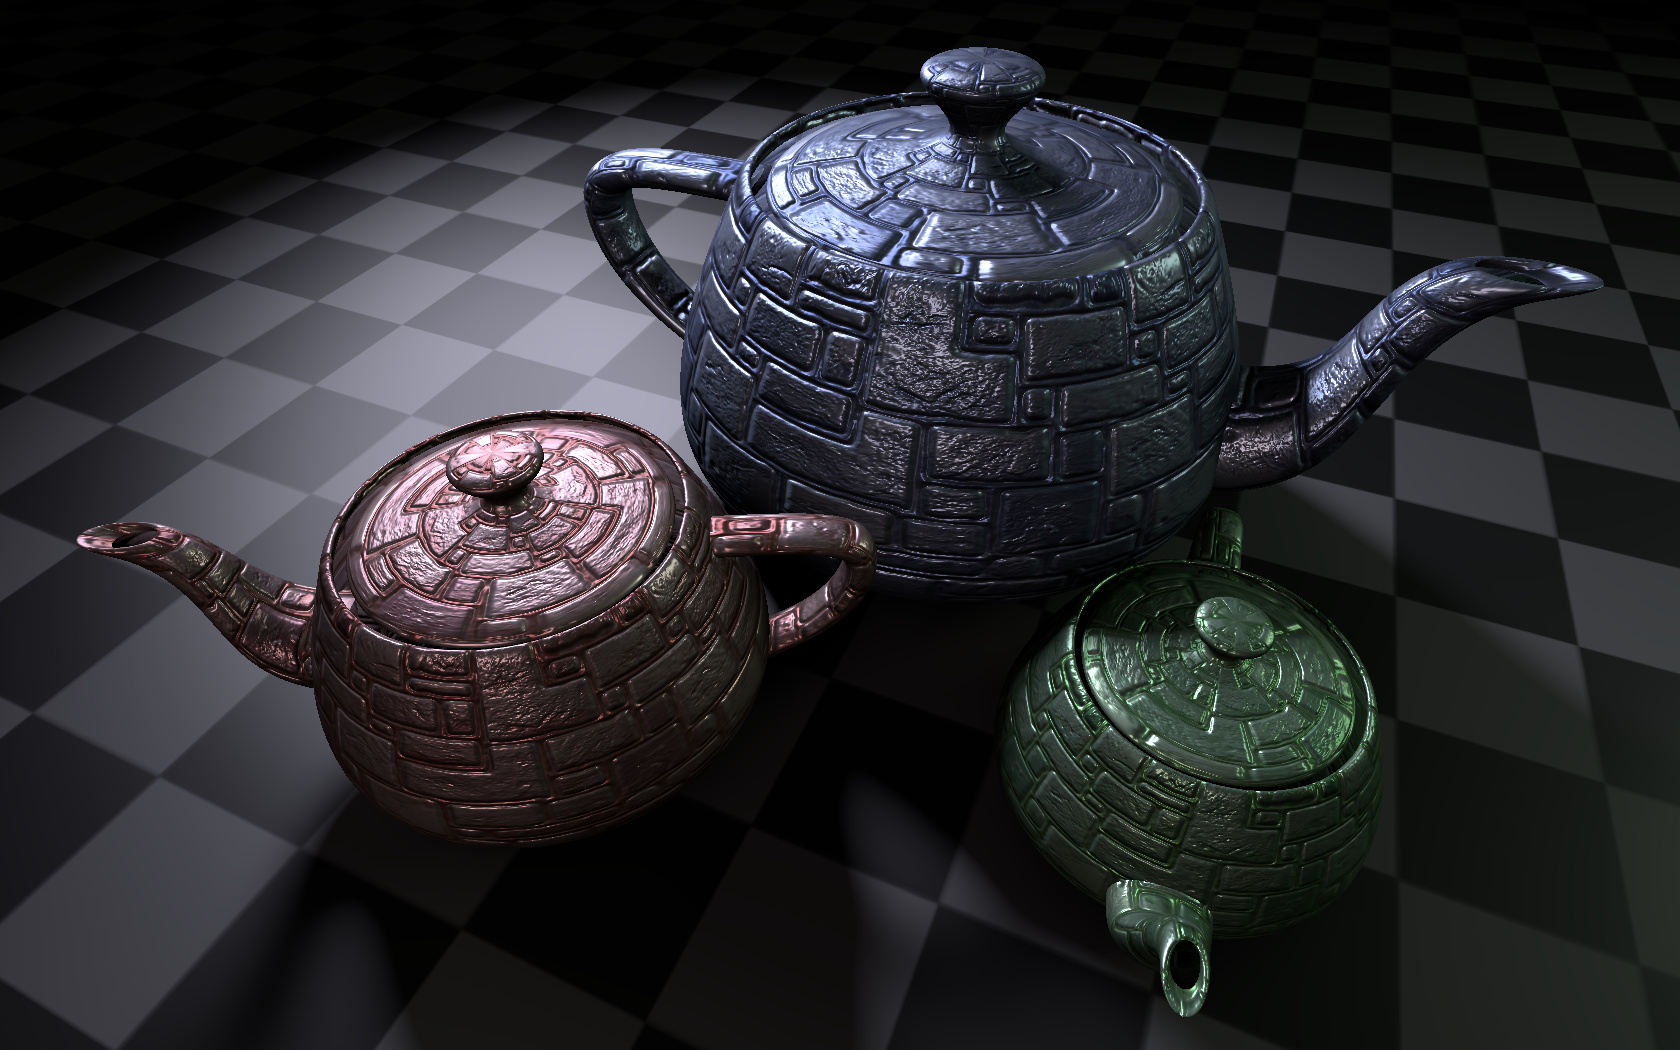
\includegraphics[width=0.45\linewidth]{./Figures/postProc/noAcuity.jpg}}
  \subfigure[Spatial acuity and color sensitivity reduction (exaggerated)]{\label{fig:postProcAcuity}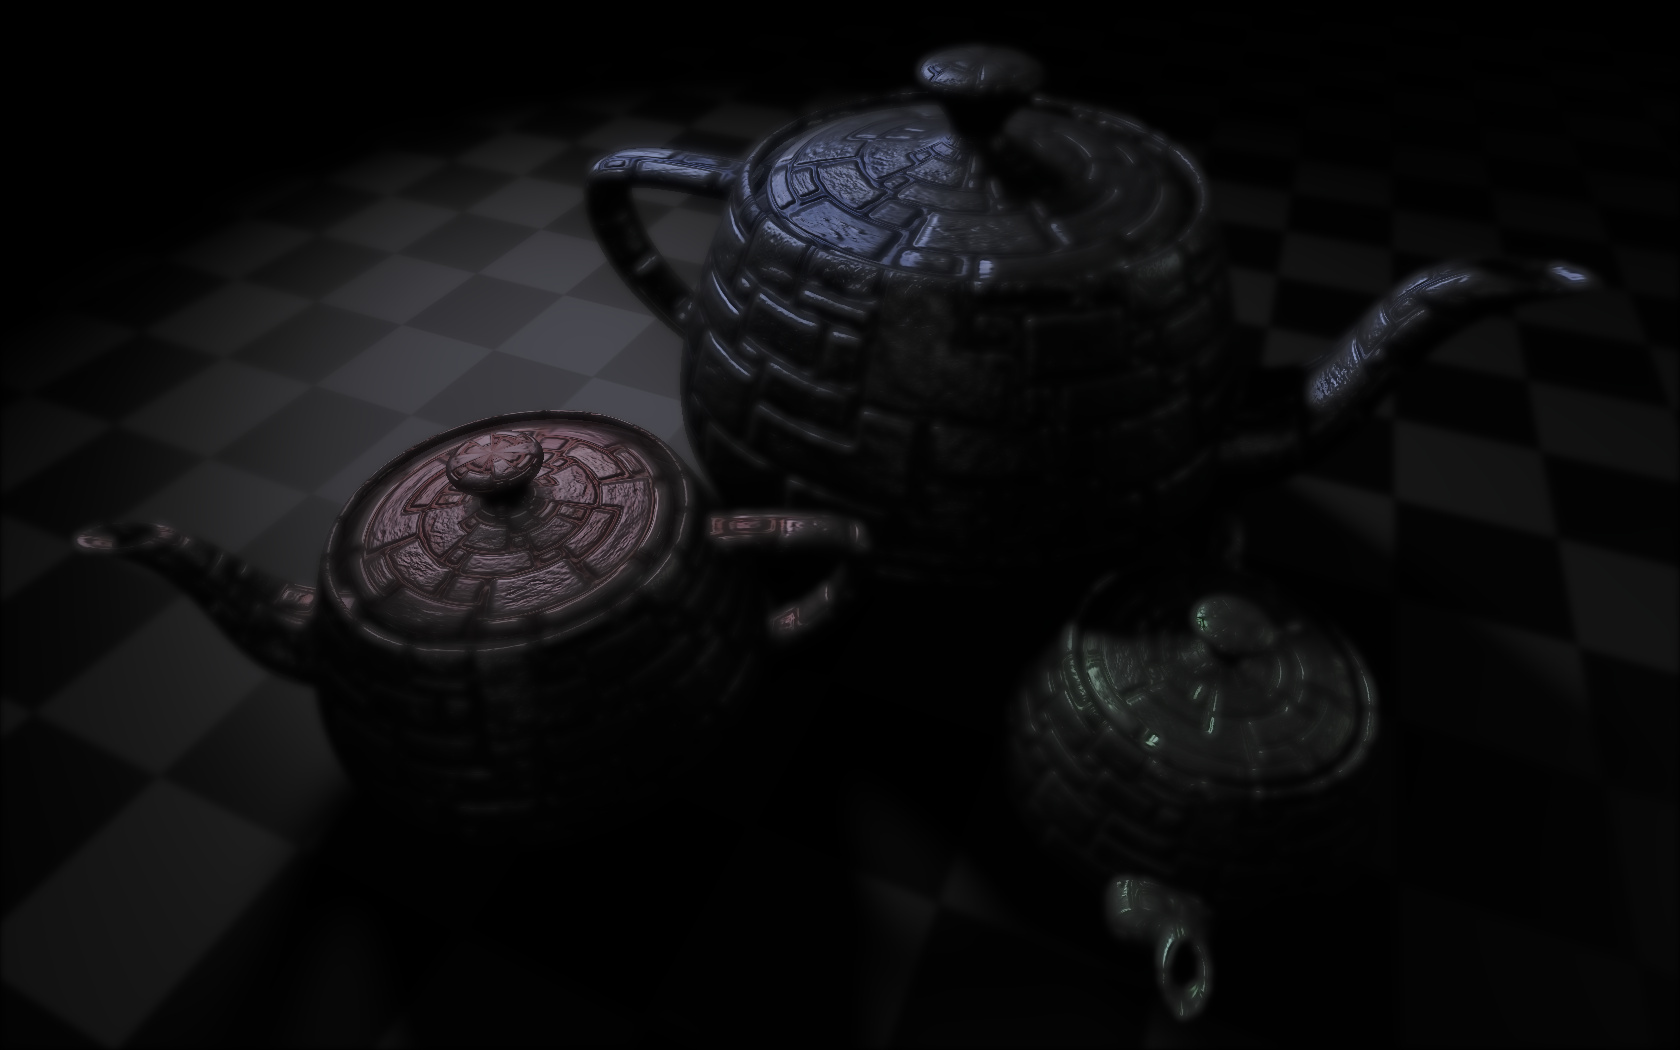
\includegraphics[width=0.45\linewidth]{./Figures/postProc/acuity.jpg}}
  \subfigure[Acuity map]{\label{fig:postProcAcuityMap}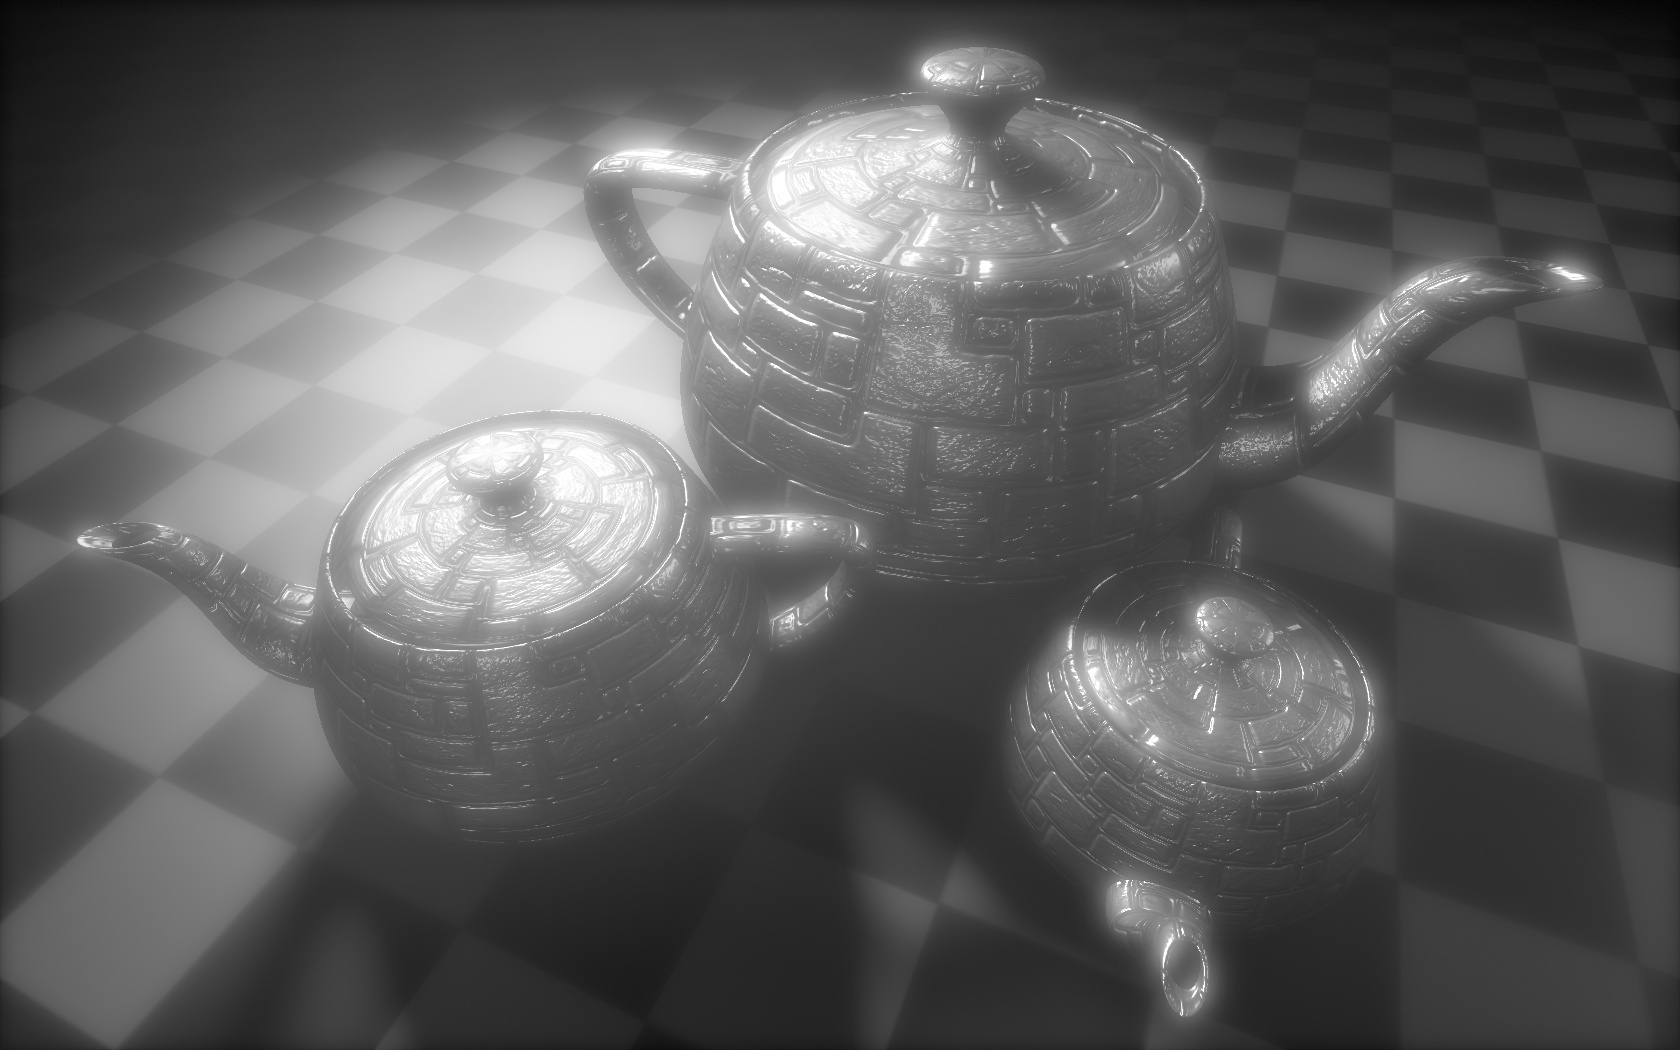
\includegraphics[width=0.45\linewidth]{./Figures/postProc/acuityMap.jpg}}
  \caption[Scotopic vision]{Realism enhancement at low-luminance conditions}
  \label{fig:postProcAcuityComparison}
\end{figure}

\subsection{Distortion}

Unlike \emph{RenderMan}'s \emph{imager} shaders, the post-processing kernels in Nucleus may freely access any pixels in the image. Another use case of this flexibility, besides blur, is the ability to distort the rendered image, either to simulate lensing phenomena or simply for an artistic purpose. For the purposes of this demonstration, the implemented example is an animated noise-based distortion.

\begin{figure}[h!]
  \centering
    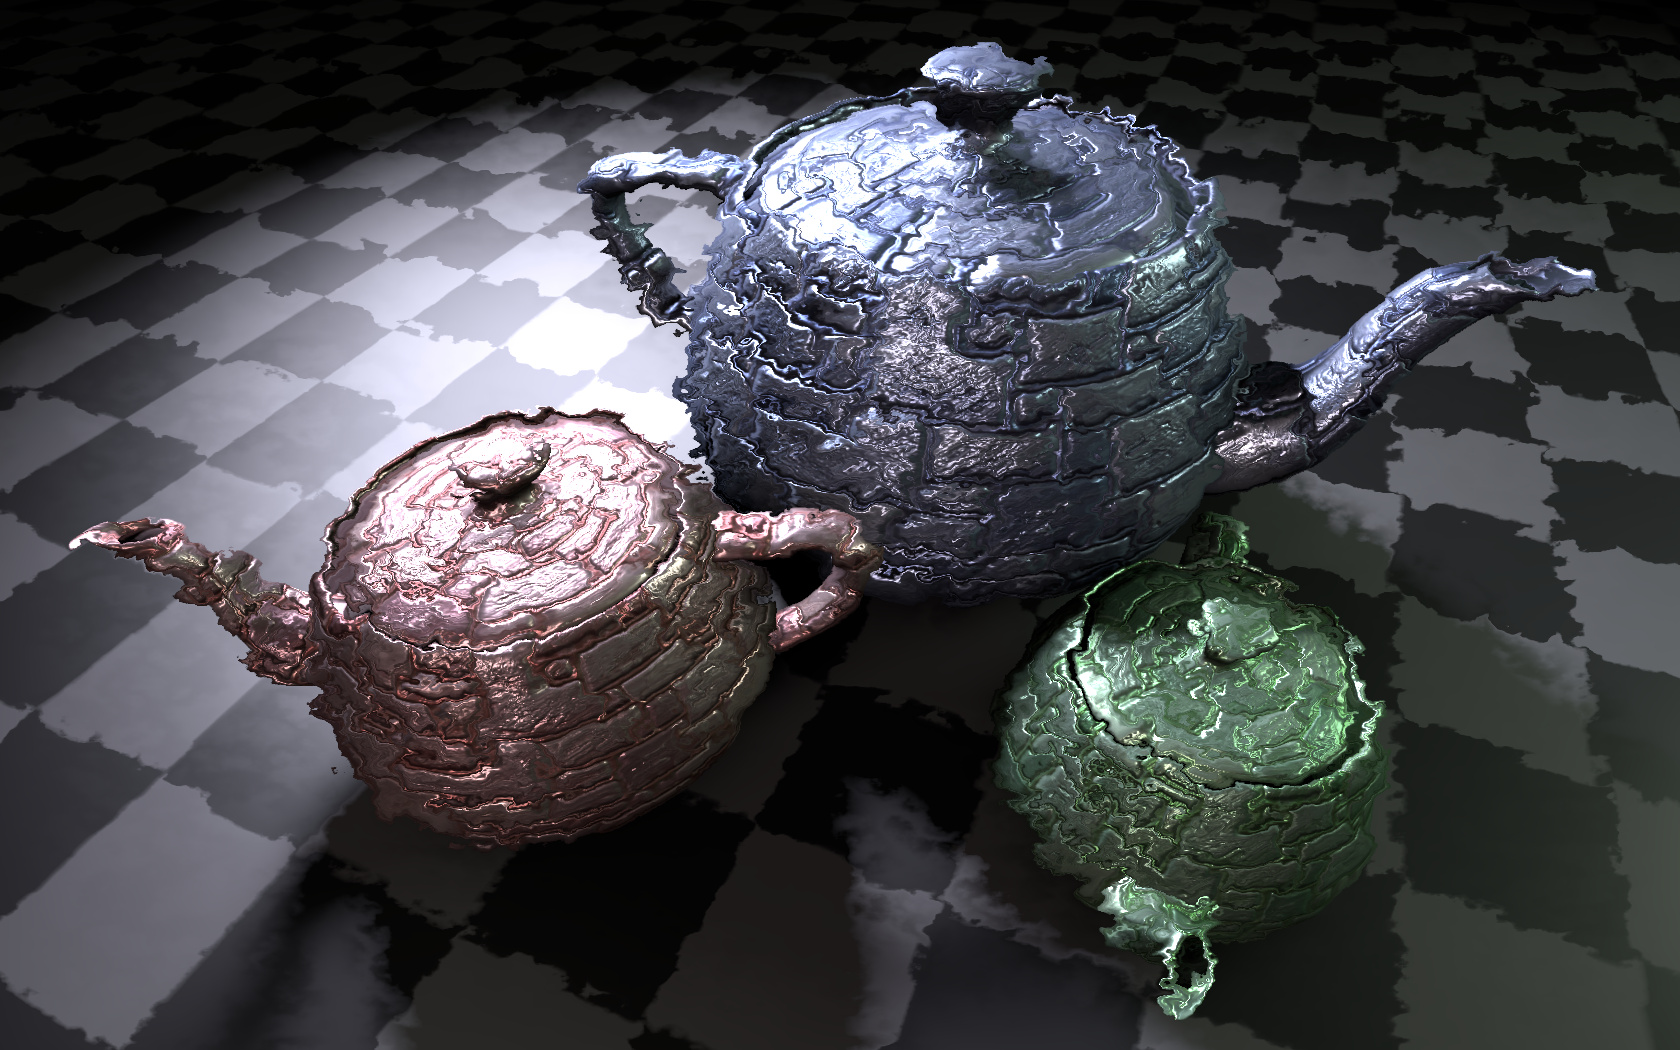
\includegraphics[width=0.9\linewidth]{./Figures/postProc/distortion.jpg}
    \caption[Distortion]{Noise-based distortion effect}
  \label{fig:postProcDistortion}
\end{figure}

An image containing Perlin noise is sampled for each pixel with a time-based offset, then passed through the cosine function and scaled to obtain an offset into the image being filtered. Additionally, smooth decay of the offsets is used near screen edges in order to avoid clamping or tiling artifacts. This is implemented by the following snippet of \emph{Cg} code:

\begin{lstlisting}[frame=single]
float2 baseOff = tex2D(distortSampler, uv * 3 + time.minute).xy * 27.123;
float2 off = cos(baseOff + radians(time.second * 360)) * 0.005;
float2 decay = smoothstep(1, 0.9, saturate(2 * abs(uv - float2(0.5))));
output = baseColor.sample(saturate(uv + off * decay));
\end{lstlisting}

The ``magic'' numbers governing offsets have been chosen arbitrarily as to define the particular look of the effect shown in figure \ref{fig:postProcDistortion}.

\subsection{Banding reduction}

Due to various limitations of display technology, it is not possible to exactly display the luminance values, even if they fall within the luminous intensity range of the target device. In particular, even if the computed values are of high precision, they need to be quantized to 8 bits per channel for final display. The situation is worsened by inexact implementation of the \textbf{sRGB} standard by monitor manufacturers. As a result, many consumer monitors cannot display even the expected 256 shades of gray. This quantization results in artifact known as ``banding'', and occurs particularly often in case of wide gradients. In three-dimensional rendering, the problem mostly occurs on flat unicolored surfaces lit from a large distance. Figure \ref{fig:postProcBanding} illustrates a part of the test scene where this happens (the lower right corner).

Since the post-processing pipeline works on high-precision values of the images, it may apply a technique known as \emph{dithering}. Dithering utilizes the intrinsic ability of the human visual system of noise removal. By diffusing the limited palette in a random (or semi-random) spatially-varying pattern, it creates the illusion of higher color depth. Historically, it has been widely used with 8- and 16-bit graphics, however it can still be utilized with ``Truecolor'' images.

The example filter adds animated signed uniform noise to the high-precision image before gamma-correction and quantization. This makes the noise most apparent in areas of low-luminosity, where banding is normally most perceivable. A single frame of the temporally-varying result can be seen in figure \ref{fig:postProcNoBanding}.

\begin{figure}[h!]
  \centering
  \subfigure[Post-processing off]{\label{fig:postProcBanding}
\includegraphics[width=0.45\linewidth]{./Figures/postProc/banding.png}}
  \subfigure[Banding hidden by noise]{\label{fig:postProcNoBanding}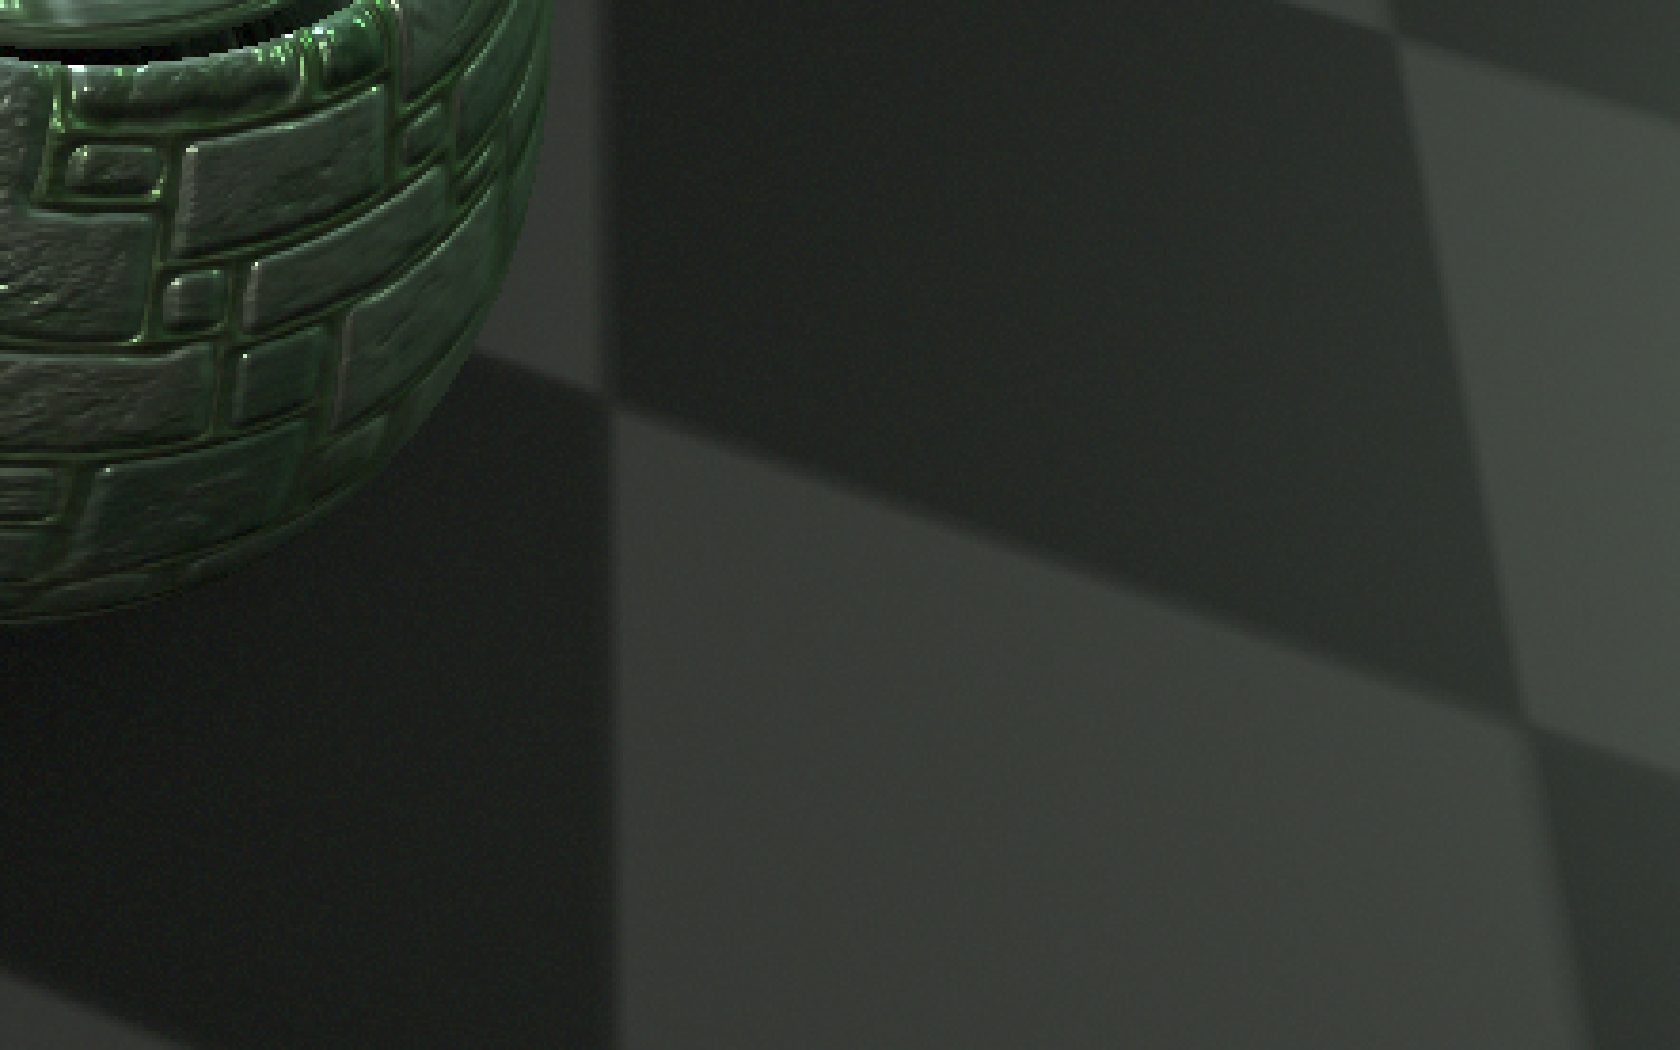
\includegraphics[width=0.45\linewidth]{./Figures/postProc/noBanding.png}}
  \caption[Color banding reduction]{Color banding reduction}
  \label{fig:postProcBandingNoBanding}
\end{figure}
